\documentclass[
    11pt, % Set the default font size, options include: 8pt, 9pt, 10pt, 11pt, 12pt, 14pt, 17pt, 20pt
    %
    aspectratio=169, % Uncomment to set the aspect ratio to a 16:9 ratio which matches the aspect ratio of 1080p and 4K screens and projectors
]{beamer}
\usepackage{mathtools}
\usepackage{caption}
\usepackage{subcaption}
\usepackage{xcolor}
\graphicspath{{Images/}{./}} % Specifies where to look for included images (trailing slash required)
\usepackage{booktabs} % Allows the use of \toprule, \midrule and \bottomrule for better rules in tables
\usepackage{bm}
%\usepackage{appendixnumberbeamer} %If you want a separate slide counter for your appendix

%%% Customize Theme %%%%%%%%%%%%%%%%%%%%%%
\usetheme{Madrid} % You can use other themes too, but this changes many things. I've found Madrid to be the best for this color scheme

%fg = font color
%bg = background color

% ! WARNING ! : Many colors are linked to multiple attributes, so changing one color can have unexpected changes!

% If you want to tweak the shading of orange and red, tweak the below 2 lines:t
\definecolor{myRed}{RGB}{120,4,4}
\definecolor{myOrange}{RGB}{227, 125, 0}

% Bottom right hand color
\setbeamercolor*{structure}{bg=myRed!20,fg=myRed!90}

\setbeamercolor*{palette primary}{use=structure,fg=white,bg=structure.fg} %?
\setbeamercolor*{palette secondary}{use=structure,fg=myRed,bg=white}
    %bottom left of footer & bar between title & top bubbles
\setbeamercolor*{palette tertiary}{use=structure,fg=white,bg=myRed} 

\setbeamercolor{frametitle}{bg=myRed!85,fg=white} %title of each slide

\setbeamercolor*{titlelike}{parent=palette primary} %?
%\setbeamercolor{titlelike}{parent=palette primary,fg=structure.fg!50!myRed}

%for miniframe (very top) AND center footer
\setbeamercolor{section in head/foot}{fg=myOrange, bg=white}

%%% Specific Colors %%%
\setbeamercolor{item projected}{bg=myOrange}
\setbeamertemplate{enumerate items}{bg=myOrange}

\setbeamercolor{itemize item}{fg=myOrange}
\setbeamercolor{itemize subitem}{fg=myOrange}

\setbeamercolor{button}{bg=myOrange}

%%% Edits ONLY the TOC slide %%%
\setbeamercolor{section in toc}{fg=black}
\setbeamercolor{subsection in toc}{fg=black}

%%% Block Colors %%%
% Standard block %
    \setbeamercolor{block title}{bg=myOrange, fg=white}
    \setbeamercolor{block body}{bg=myOrange!20}

% Alerted block % If you want to customize it's color
    %\setbeamercolor{block title alerted}{bg=cyan, fg=white}
    %\setbeamercolor{block body alerted}{bg=cyan!10}

% Example block % If you want to customize it's color
    %\setbeamercolor{block title example}{bg=cyan, fg=white}
    %\setbeamercolor{block body example}{bg=cyan!10}

%---------------------------------------------------------
%	SELECT FONT THEME & FONTS
%---------------------------------------------------------
\usefonttheme{default} % Typeset using the default sans serif font
\usepackage{palatino} % Use the Palatino font for serif text
\usepackage[default]{opensans} % Use the Open Sans font for sans serif text
\useinnertheme{circles}

%---------------------------------------------------------
%	SELECT OUTER THEME
%---------------------------------------------------------
% Outer themes change the overall layout of slides, such as: header and footer lines, sidebars and slide titles. Uncomment each theme in turn to see what changes it makes to your presentation.

%\useoutertheme{default}
%
\useoutertheme{miniframes}

%\useoutertheme{infolines}
%\useoutertheme{smoothbars}
%\useoutertheme{sidebar}
%\useoutertheme{split}
%\useoutertheme{shadow}
%\useoutertheme{tree}
%\useoutertheme{smoothtree}

%---------------------------------------------------------
%	PRESENTATION INFORMATION
%---------------------------------------------------------
\logo{
\includegraphics[width=1cm]{Images/logo_ib.jpg}}
\title[Descripción del efecto de inducción cromática]{Descripción teórico-experimental del efecto de inducción cromática}
\subtitle{Defensa de Tesis de Maestría}
%\author[Segovia]{Autor: Tadeo N. Segovia}
\author[Tadeo N. Segovia]{Tadeo N. Segovia\\{\small Directora: Inés Samengo}\\{\small Colaborador: Nicolás Vattuone}}

%\author[Inés Samengo]{Author: Inés Samengo}
\institute[]{ Jurado: \\
M. Onetto, E. Kropff, G. Rozas \\
\vspace{0.5cm}
    Instituto Balseiro, Universidad Nacional de Cuyo \\
 Departamento de Física Médica, Centro Atómico Bariloche \\
}


\date[19/12/2023]
%\date[\today]


%\DeclareUnicodeCharacter{0301}{*************************************}

%---------------------------------------------------------
%---------------------------------------------------------
%---------------------------------------------------------
\begin{document}

%---------------------------------------------------------
%	TITLE SLIDE
%---------------------------------------------------------
\section{}
\begin{frame}
	\titlepage % Output the title slide, automatically created using the text entered in the PRESENTATION INFORMATION block above
\end{frame}

%---------------------------------------------------------
%	TABLE OF CONTENTS SLIDE
%---------------------------------------------------------
% The table of contents outputs the sections and subsections that appear in your presentation, specified with the standard \section and \subsection commands. You may either display all sections and subsections on one slide with \tableofcontents, or display each section at a time on subsequent slides with \tableofcontents[pausesections]. The latter is useful if you want to step through each section and mention what you will discuss.

%\begin{frame}
%	\frametitle{Table of contents} % Slide title, remove this command for no title
	
%	\tableofcontents % Output the table of contents (all sections on one slide)
	%\tableofcontents[pausesections] % Output the table of contents (break sections up across separate slides)
%\end{frame}


%---------------------------------------------------------
%	PRESENTATION BODY SLIDES
%---------------------------------------------------------
    \section{Introducción} % Sections are added in order to organize your presentation into discrete blocks, all sections and subsections are automatically output to the table of contents as an overview of the talk but NOT output in the presentation as separate slides

%------------------------------------------------
\begin{frame}
	\frametitle{Inducción cromática}
            


\begin{columns}[c] % The "c" option specifies centered vertical alignment while the "t" option is used for top vertical alignment
		\begin{column}{0.4\textwidth} % Right column width
                \begin{itemize}
                    \item \onslide<1-> 
                    Cambio en el color de un dado estímulo originado por la cromaticidad de su entorno.\newline 
                    \item \onslide<2->
                    El efecto es repulsivo, el cambio intensifica el contraste entre el color del estímulo y su entorno.
                \end{itemize}
                
                
		\end{column}
  		\onslide<1->\begin{column}{0.6\textwidth} % Left column width
                \begin{figure}
                    \centering
                    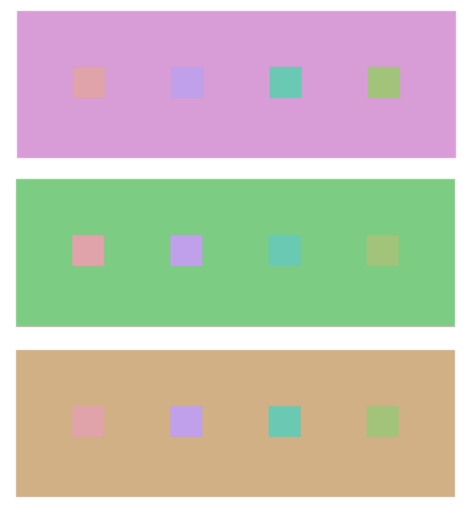
\includegraphics[width=4.5cm]{Images/intro/ind_crom_ej.PNG}
                    %\caption{Caption}
                    %\label{fig:my_label}
                \end{figure}
		\end{column}
	\end{columns}


\end{frame}

%------------------------------------------------


%------------------------------------------------




%--------------------------------------------------

%-------------------------------------------------

%------------------------------------------------
\begin{frame}{Objetivos}
    \begin{itemize}
        \item<1-> \textbf{Desarrollamos una descripción teórica del proceso de inducción cromática que contiene parámetros anatómicos y fisiológicos de las redes neuronales subyacentes.}
        \item<2-> \textbf{Diseñamos y llevamos a cabo experimentos comportamentales en una población de voluntarios que permiten acceder a estos parámetros.}
    \end{itemize}
\end{frame}





%------------------------------------------------
\section{Desarrollo teórico}



%----------------------------------------------------
\begin{frame}{Introducción}{Pathway visual}
 % The "c" option specifies centered vertical alignment while the "t" option is used for top vertical alignment

% Left column width
         \onslide<1-> \begin{figure}[h!]
            \centering
            %\caption{Hawkins et al, 2015}
            \includegraphics[angle=0, width=13cm]{Images/intro/esquema_visual_pathaway_horizontal.pdf}
         \end{figure}
	
\end{frame}


\begin{frame}{Introducción}{Pathway visual}
    \begin{itemize}
                    \item \onslide<1-> La información transmitida por las células ganglionares codifica la composición lumínica y cromática de un cierto área del campo visual.
                    \item \onslide<2-> Esto se debe, entre otras cosas, a las conexiones laterales causadas por las células
                    horizontales y amácrinas, y a la convergencia que se observa en la transmisión feedfoward fotorreceptores $\rightarrow$ bipolares $\rightarrow$ ganglionares. 
                    \item \onslide<3-> Son estas conexiones las que vuelven a la percepción del estímulo dependiente de su entorno.
    \end{itemize} \end{frame}
    
\begin{frame}{Introducción}{Campos receptivos}
 \begin{columns}[c] % The "c" option specifies centered vertical alignment while the "t" option is used for top vertical alignment

    
		\begin{column}{0.45\textwidth}
  El procesamiento de información visual en la retina puede ser modelado como un filtro lineal $\mathbf{G}$ conocido como \emph{campo receptivo}.\newline
          \begin{equation*}
    O(\mathbf{x}) = \displaystyle\int \mathop{d\mathbf{x'}} \mathbf{G}(\mathbf{x},\mathbf{x}') L(\mathbf{x'})
\end{equation*}\newline
 
               
		\end{column}
  		\begin{column}{0.55\textwidth} % Left column width
                \onslide<1-> \begin{figure}[h!]
                    \centering
                    %\caption{Hawkins et al, 2015}
                    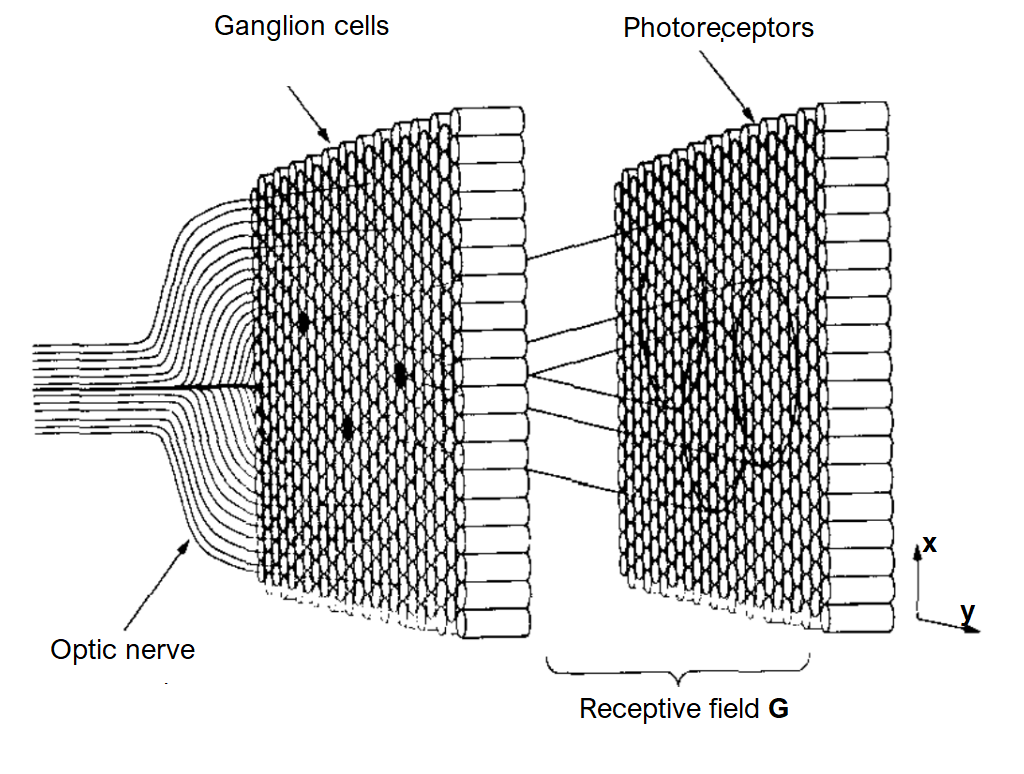
\includegraphics[angle=0, width=5.5cm]{Images/intro/esquema_campo_receptivo.PNG}
                    %\label{Figure 1}
                \end{figure}
		\end{column}		
	\end{columns}
        \end{frame}


\begin{frame}{Introducción}{Estructura center-surround}
    \begin{columns}[c] % The "c" option specifies centered vertical alignment while the "t" option is used for top vertical alignment

    
		\begin{column}{0.45\textwidth}

Los campos receptivos de las células de la retina suelen tener estructura \emph{center-surround}.
Es decir, las neuronas de la primera capa ubicadas en $\mathbf{x}'$ cercanos a la neurona de la segunda capa ubicada en $\mathbf{x}$ la afectan positivamente y 
aquellas ubicadas en $x'$ lejanos la afectan negativamente (o viceversa).
 
               
		\end{column}
  		\begin{column}{0.55\textwidth} % Left column width
                \onslide<1-> \begin{figure}[h!]
                    \centering
                    %\caption{Hawkins et al, 2015}
                    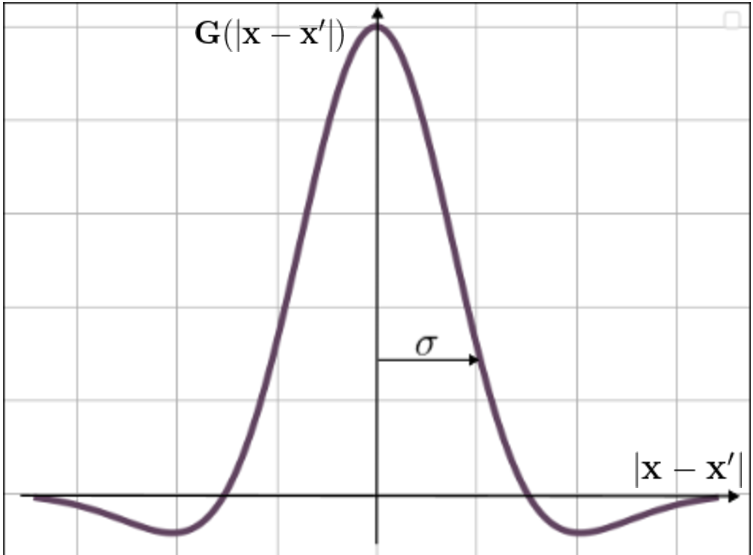
\includegraphics[angle=0, width=5.5cm]{Images/intro/center_surrond.pdf}
                    %\label{Figure 1}
                \end{figure}
		\end{column}		
	\end{columns}
\end{frame}



%------------------------------------------------
\begin{frame}{Introducción}
	\framesubtitle{Coordenadas perceptuales}
    %\framesubtitle{Coordenadas perceptuales}

  \begin{columns}[c] % The "c" option specifies centered vertical alignment while the "t" option is used for top vertical alignment

    
		\begin{column}{0.45\textwidth} % Right column width
                \begin{itemize}
                    \item \onslide<1-> En un trabajo $\text{anterior}^1$ se describió el efecto de inducción cromática como un desplazamiento en el espacio de colores.
                    \item \onslide<2-> Se demostró que existe un sistema de coordenadas donde este efecto es isotrópico y homogéneo. 
                    \item \onslide<3->Llamamos a este sistema de coordenadas como  \emph{coordenadas perceptuales}.
                \end{itemize}
        
               
		\end{column}
  		\begin{column}{0.55\textwidth} % Left column width
                \onslide<1-> 

                \begin{figure}
                    \centering
                    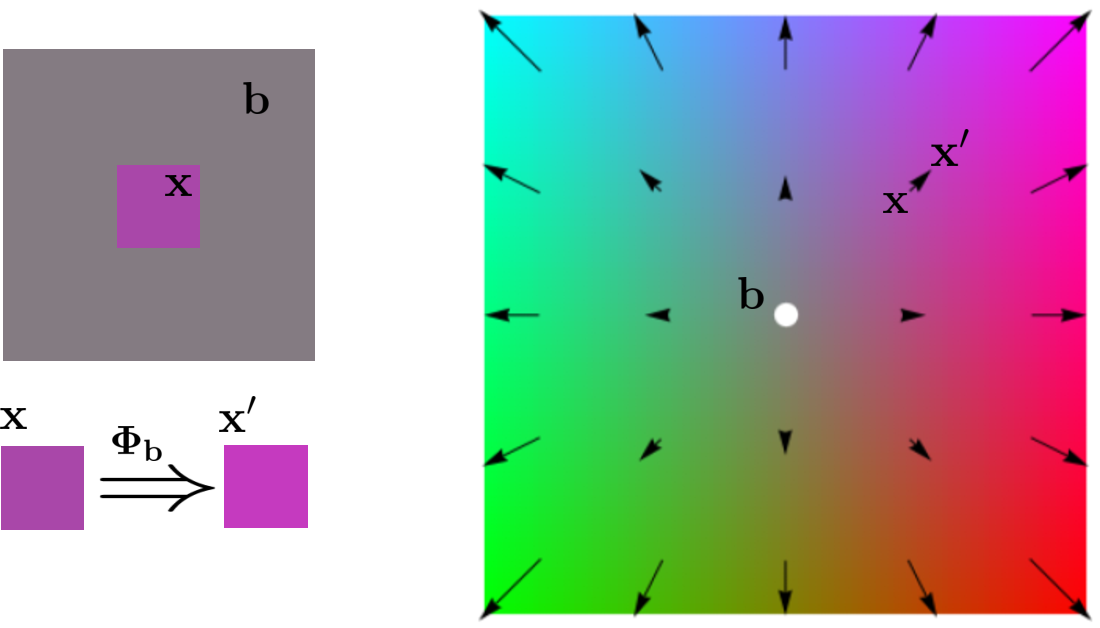
\includegraphics[width = 7cm]{Images/intro/repulsion.pdf}
                    %\caption{Caption}
                    %\label{fig:enter-label}
                \end{figure}
                
                %\begin{figure}[h!]
                 %   \centering
                 %   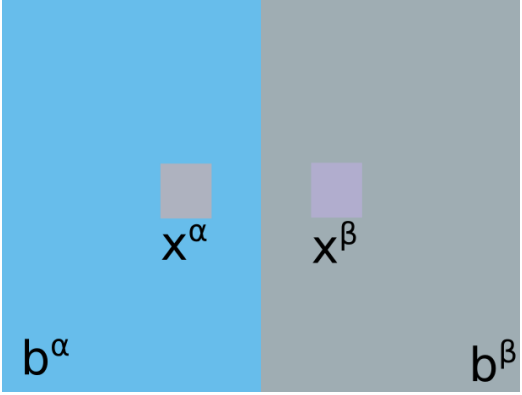
\includegraphics[angle=0, width=2.5cm]{Images/teorico/ejemplo.PNG}
                    %\caption{}
                    %\label{fig:my_label}
                %\end{figure}
                %\begin{figure}[h!]
                 %   \centering
                    %\caption{Hawkins et al, 2015}
                 %   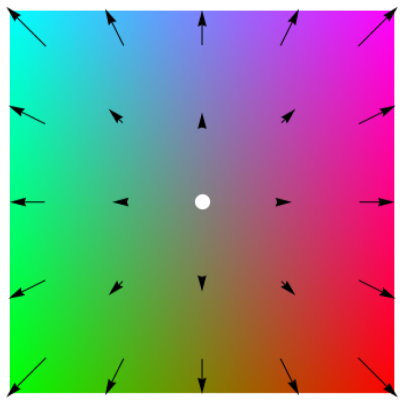
\includegraphics[angle=0, width=2.7cm]{Images/intro/fig0.png}
                    %\label{Figure 1}
                %\end{figure}
		\end{column}		
	\end{columns}

        
        
\end{frame}



\begin{frame}{Trabajo previo}
 \begin{columns}[c] % The "c" option specifies centered vertical alignment while the "t" option is used for top vertical alignment

    
		\begin{column}{0.45\textwidth}
  
  El color de un estímulo en la posición $x$ está representada por $\mathbf{r}(x)$, sus coordenadas en el espacio de colores.\newline
          
 
               
		\end{column}
  		\begin{column}{0.55\textwidth} % Left column width
                \onslide<1-> \begin{figure}[h!]
                    \centering
                    %\caption{Hawkins et al, 2015}
                    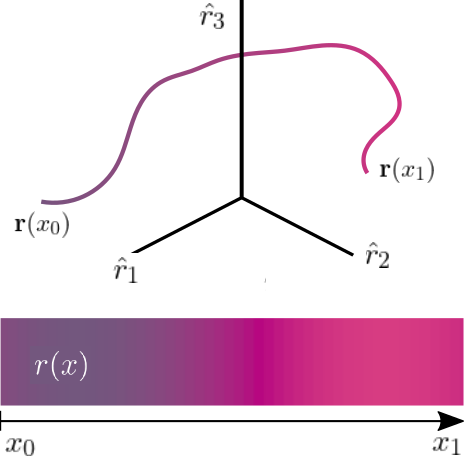
\includegraphics[angle=0, width=5.5cm]{Images/que_es_r_x.png}
                    %\label{Figure 1}
                \end{figure}
		\end{column}		
	\end{columns}
\end{frame}






\begin{frame}
	\frametitle{Trabajo previo}
    \framesubtitle{El efecto del campo receptivo sobre el estímulo cromático}

    El color percibido $ \mathbf{\tilde{r}}(\mathbf{x})$ es una versión filtrada del estímulo físico $\mathbf{r}(\mathbf{x})$, producto de un campo receptivo cromático $\mathbf{G}$.
    %We work with chromaticities processed by a time-independent receptive field $\mathbf{G}(\mathbf{x},\mathbf{x}')$ 

        
    \begin{equation*}
    \mathbf{\tilde{r}}(\mathbf{x}) = \displaystyle \int \mathop{d\mathbf{x}'}   \mathbf{G}(\mathbf{x},\mathbf{x}') \mathbf{r}(\mathbf{x}')
\end{equation*}
\small 
$\mathbf{x} \Rightarrow$  Coordenadas espaciales\\
$\mathbf{r} \Rightarrow$ Coordenadas perceptuales de la cromaticidad estímulo.\\
$\mathbf{\tilde{r}} \Rightarrow$ Coordenadas perceptuales del color del estímulo.
\normalsize


 

\end{frame}




%------------------------------------------------
\begin{frame}{Desarrollo teórico}
    \framesubtitle{El efecto del campo receptivo sobre el estímulo cromático}
    Utilizando la invarianza traslacional de los campos receptivos convolucionales
 \begin{equation*}
     \mathbf{\tilde{r}}(\mathbf{x}) = \displaystyle \int \mathop{d\mathbf{x}'}   \mathbf{G}(\mathbf{x},\mathbf{x}') \mathbf{r}(\mathbf{x}') \,\Rightarrow\, \mathbf{\tilde{r}}(\mathbf{x}) = \displaystyle \int \mathop{d\mathbf{x}'}   \mathbf{G}(\mathbf{x}-\mathbf{x}') \mathbf{r}(\mathbf{x}')
\end{equation*}
\end{frame}
%If the stimulus has uniform chromaticity there must be no shift in the perceived color, i.e., 
%\begin{equation*}
 %   \int \mathop{d\mathbf{x}'} \mathbf{G}(\mathbf{x}') = 1.
%\end{equation*} 



%----------------------------------------------
\begin{frame}{Trabajo previo}
    En las coordenadas perceptuales, la inducción cromática tiene simetría rotacional, es decir, si
$\vec{r}$ es transformado por una rotación arbitraria $\mathcal{R}$, entonces $\vec{\tilde{r}}$ debe transformar de la misma manera. por lo tanto $\mathbf{G}$ debe ser una matriz escalar
\begin{equation*}
     \mathbf{G}(\mathbf{x}-\mathbf{x}') = \textit{G}(\mathbf{x}-\mathbf{x}') \, \mathbf I_3 
\end{equation*}
\begin{figure}
    \centering
    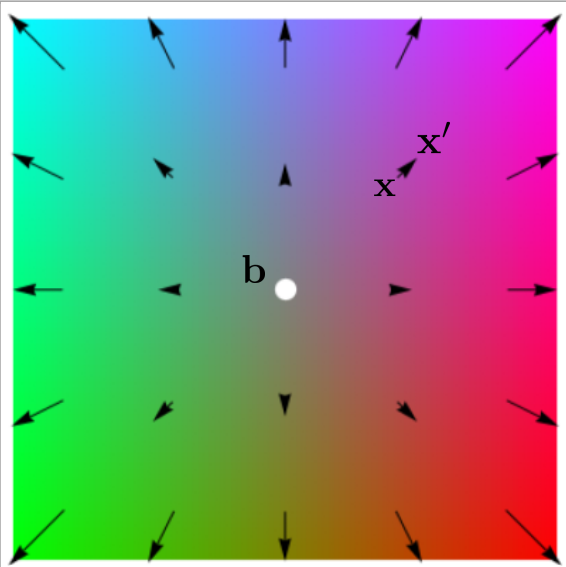
\includegraphics[width = 4cm]{Images/intro/solo_radial.png}
\end{figure}
\end{frame}

%-------------------------------------------------


\begin{frame}{Trabajo previo}
    \framesubtitle{Input sinusoidal unidimensional}
    Si presentamos el estímulo $\mathbf{r}(x)$, 
    obtenemos el color $\mathbf{\tilde{r}}(x)$
    \onslide<1->\begin{equation*}
 \mathbf{r} = \displaystyle\frac{\mathbf{r}_0 + \mathbf{r}_1}{2} + \displaystyle\frac{\mathbf{r}_0 - \mathbf{r}_1}{2}\cos{(kx)} \xRightarrow{\mathbf{G}} \mathbf{\tilde{r}} = \displaystyle\frac{\mathbf{r}_0 + \mathbf{r}_1}{2} + \displaystyle\frac{\mathbf{r}_0 - \mathbf{r}_1}{2}\cos{(kx)} \color{red} \, \mathcal{F}[\mathbf{G}](k)
\end{equation*}


\begin{figure}
    \centering
    
\includegraphics[width = 10cm]{Images/coseno_estimulo_y_amplificado.png}
    %\caption{Caption}
    %\label{fig:my_label}
\end{figure}




%\begin{figure}
 %   \centering
 %   
\includegraphics[width = 9cm]{franja.PNG}
    %\caption{Caption}
    %\label{fig:my_label}
%\end{figure}

%\onslide<2-> 
%Obtenemos información sobre la transformada de Fourier del campo receptivo $\mathbf{G}$.
\end{frame}

%----------------------------------------------------------

\begin{frame}{Trabajo previo}
    \framesubtitle{Input sinusoidal unidimensional}
\begin{itemize}
    \item La discriminación es óptima cuando la amplitud de la modulación es máxima, es decir, cuando $\mathcal{F}[\mathbf{G}](k)$ es máxima. \newline
    \item La distancia característica $\sigma$ de $\mathbf{G}$ está relacionada con la frecuencia espacial $k$ donde $\mathcal{F}[\mathbf{G}](k)$ alcanza su máximo.
\end{itemize}   

\begin{figure}
    \centering
    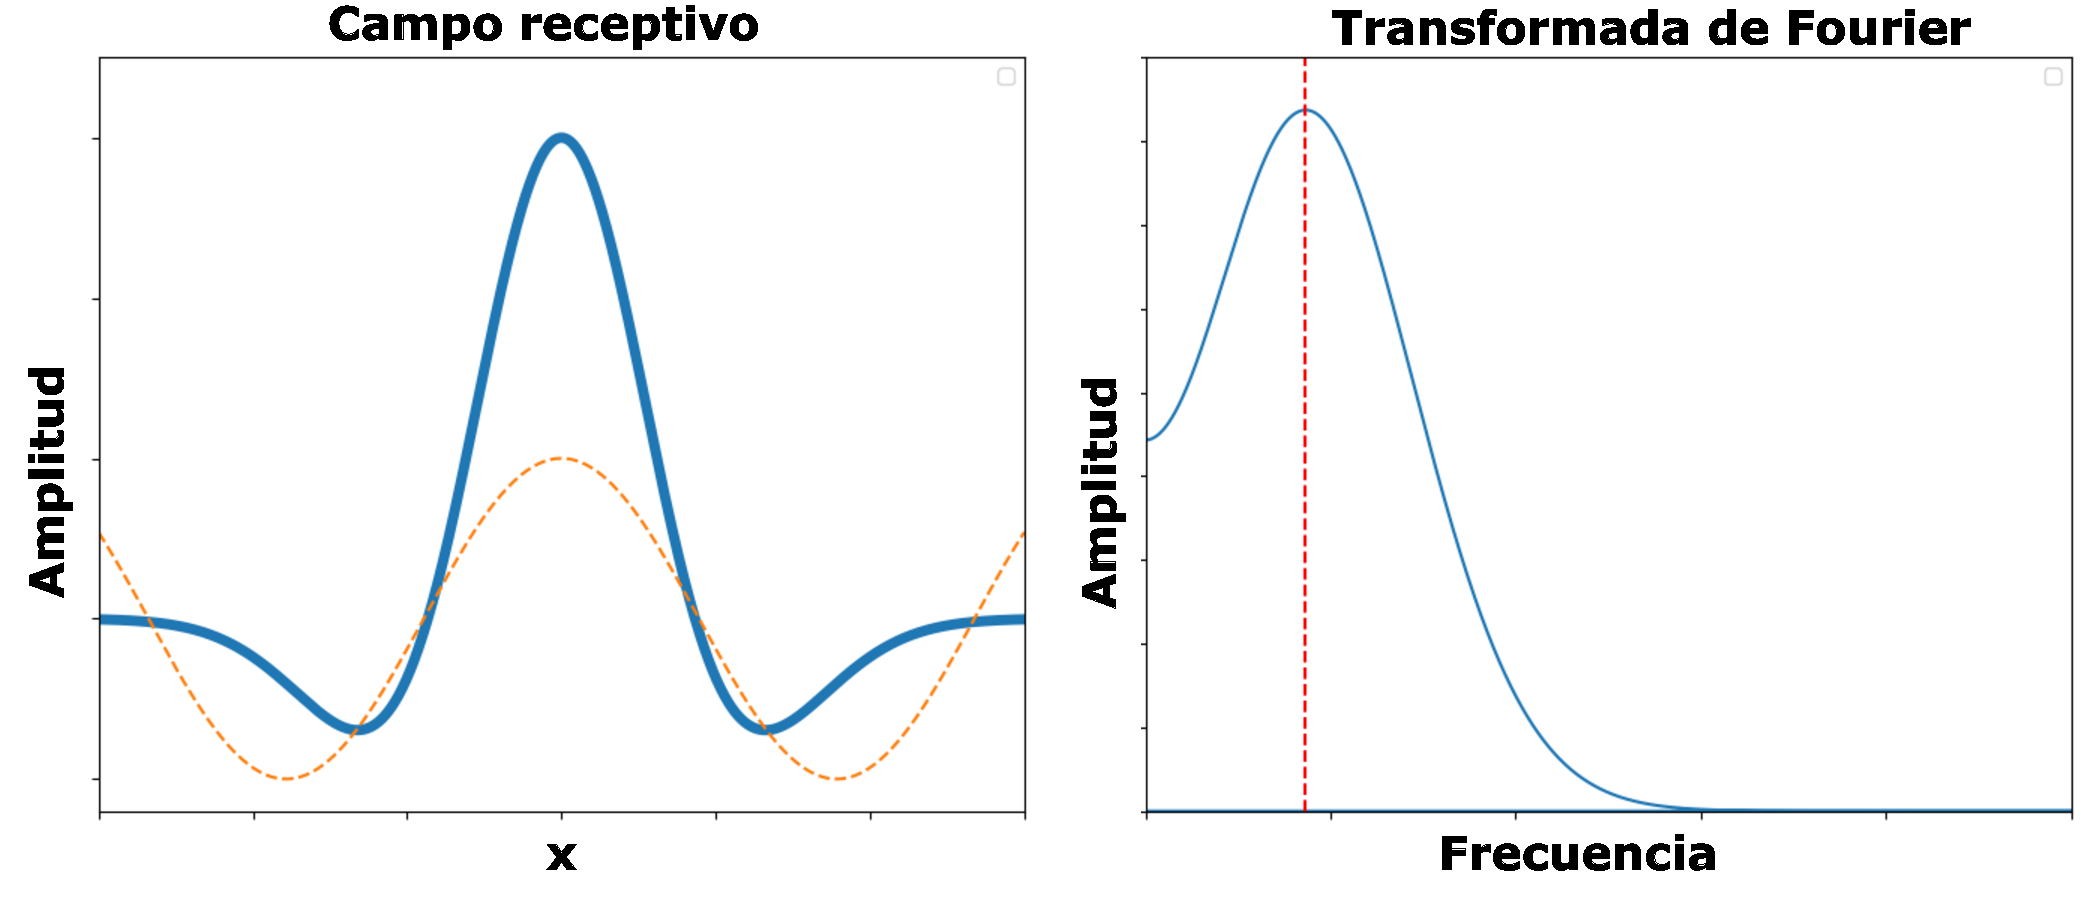
\includegraphics[width = 8.5cm]{Images/intro/fourier_transform_def.pdf}
    %\caption{Caption}
    %\label{fig:my_label}
\end{figure}



\end{frame}




%------------------------------------------------
%\begin{frame}{Trabajo previo}
 %   \framesubtitle{Input sinusoide 1D}
 %   The perceived color is
%\onslide<1->$\mathbf{\tilde{r}} = \displaystyle\int \mathop{dx'} \mathbf{G}(x')\frac{\mathbf{r}_0 + \mathbf{r}_1}{2} + \displaystyle \int \mathop{dx'} \mathbf{G}(x') \displaystyle\frac{\mathbf{r}_0 - \mathbf{r}_1}{2}\cos{\left[k(x-x')\right]}$\newline
%\onslide<2->That means

%\begin{equation*}
%\begin{split}
 %   \mathbf{\tilde{r}} &= \displaystyle\frac{\mathbf{r}_0 + \mathbf{r}_1}{2} + \displaystyle\frac{\mathbf{r}_0 - \mathbf{r}_1}{2}\cos(kx)\displaystyle \int \mathop{dx'} \mathbf{G}(x') \cos{\left(kx'\right)} \\
   % &= \displaystyle\frac{\mathbf{r}_0 + \mathbf{r}_1}{2} + \displaystyle\frac{\mathbf{r}_0 - \mathbf{r}_1}{2}\cos(kx) \mathcal{F}[\mathbf{G}](k)
%\end{split}
%\end{equation*}
%\onslide<3-> 
%We can get information about the receptive field $\mathbf{G}$ through its Fourier transform.
%\end{frame}

%-------------------------------------------------
\begin{frame}{Desarrollo teórico}
    \onslide<1->\framesubtitle{Caso bidimensional}
    Estamos interesados en encontrar una versión bidimensional del estímulo previo, que nos pueda servir para campos receptivos radialmente simétricos.\newline
    \onslide<2->La transformada de Hankel de orden cero está definida como   \begin{equation*}
        \boxed{\mathcal{H}[f](k) =  \displaystyle\int_0^{\infty} f(r)\, \text{J}_0(k r)\, r \mathop{dr}}
    \end{equation*}\newline
    \onslide<3->Para una función radial $f(x,y)$ , $\mathcal{H}[f](k)$ y $\mathcal{F}[f](u,v)$ están relacionadas por
    \begin{equation*}
         \boxed{\mathcal{F}_{x,y}[f](u,v) = 2\pi \mathcal{H}[f](k), \text{  con  } k = 2\pi \displaystyle\sqrt{u^2+v^2}}
    \end{equation*}
    
     
     

\end{frame}
%---------------------------------------------------
\begin{frame}{Desarrollo teórico}
\framesubtitle{Teorema de la convolución}
Usando la relación entre $\mathcal{H}[f](k)$ y $\mathcal{F}[f](u,v)$, podemos obtener una expresión similar al teorema de la convolución para $\mathcal{H}[f](k)$
\begin{equation*}
    \boxed{\mathcal{H}[f*g](k) = \mathcal{H}[f](k)\,\mathcal{H}[g](k)}
\end{equation*}


\end{frame}
%-------------------------------------------------
\begin{frame}{Desarrollo teórico}
\framesubtitle{Utilizando la función $\text{J}_0$ de Bessel como estímulo}
    Si presentamos el estímulo $\mathbf{r}(x,y)$, obtenemos el color percibido $\mathbf{\tilde{r}}$
    \begin{equation*}
        \mathbf{r} =  \mathbf{r_0} + \sqrt{k}\color{red}\bm{\epsilon}\color{black}\, \text{J}_0 \left(k\rho\right) \xRightarrow{\mathbf{G}} \mathbf{\tilde{r}} = \mathbf{r_0} + \sqrt{k}\color{red}\mathcal{H}[\mathbf{G}](k)\bm{\epsilon}\color{black} \, \,\text{J}_0\left(k\rho\right)  
    \end{equation*}

\begin{figure}
    \centering
    
\includegraphics[width = 10cm]{Images/j0_estimulo_y_amplificada.png}
    %\caption{Caption}
    %\label{fig:my_label}
\end{figure}

\end{frame}
%------------------------------------------------
%\begin{frame}{Desarrollo teórico}
%\framesubtitle{Utilizando la función $\text{J}_0$ de Bessel como estímulo}
%    \onslide<1->\begin{equation*}
%    \mathbf{\tilde{r}}(x,y) = \mathbf{r_0} +  \sqrt{k}\bm{\epsilon}\,\mathcal{H}[\mathbf{G}](k) \text{J}_0\left(k\sqrt{x^2+y^2}\right)
%\end{equation*}

%    \onslide<1->\vspace{1cm} La modulación está amplificada por $\mathcal{H}[\mathbf{G}](k)$.
    
%    \onslide<2-> \vspace{0.4cm} Podemos diseñar experimentos que nos permitan encontrar la frecuencia espacial $k$ donde la discriminación es óptima e identificar la distancia característica $\sigma$ de $\mathbf{G}$.
   
%\end{frame}


\begin{frame}{Umbral de discriminación y la distancia característica del campo receptivo}
\begin{itemize}
    \item El umbral de discriminación $h$ está relacionado a la amplitud mínima $\epsilon$ que necesita un estímulo para ser percibido.
    \item Para nuestro estímulo, este umbral está inversamente relacionado a la amplitud percibida $\color{red}\mathcal{H}[\mathbf{G}](k)$.
    \item $h(k)$ alcanza su mínimo en la frecuencia espacial $k$ donde $\mathcal{H}[\mathbf{G}](k)$ alcanza su máximo.
\end{itemize}

\onslide<2->\begin{block}{}
    
   \emph{Podemos diseñar experimentos de discriminación que nos permitan acceder al umbral de discriminación $h(k)$ para distintas frecuencias.}
    	\end{block}

\end{frame}



%------------------------------------------------
\section{Experimentos de discriminación}

%------------------------------------------------
\begin{frame}{Experimentos de discriminación}{Coordenadas LMS}
    \begin{columns}[c] % The "c" option specifies centered vertical alignment while the "t" option is used for top vertical alignment

    
		\begin{column}{0.45\textwidth}

    \begin{itemize}
        \item Cada coordenada esta asociada con la señal absorbida por cada tipo de cono en la retina.
        \item Combinaciones lineales de estas coordenadas están asociadas a propiedades cromáticas (\textbf{L - M} y \textbf{S}) y lumínicas de los \\ estímulos (\textbf{L + M}).
        \item Son reproducibles a diferencia de las coordenadas \textbf{RGB}.
    \end{itemize}

          
 
               
		\end{column}
  		\begin{column}{0.55\textwidth} % Left column width
                \onslide<1-> \begin{figure}[h!]
                    \centering
                    %\caption{Hawkins et al, 2015}
                    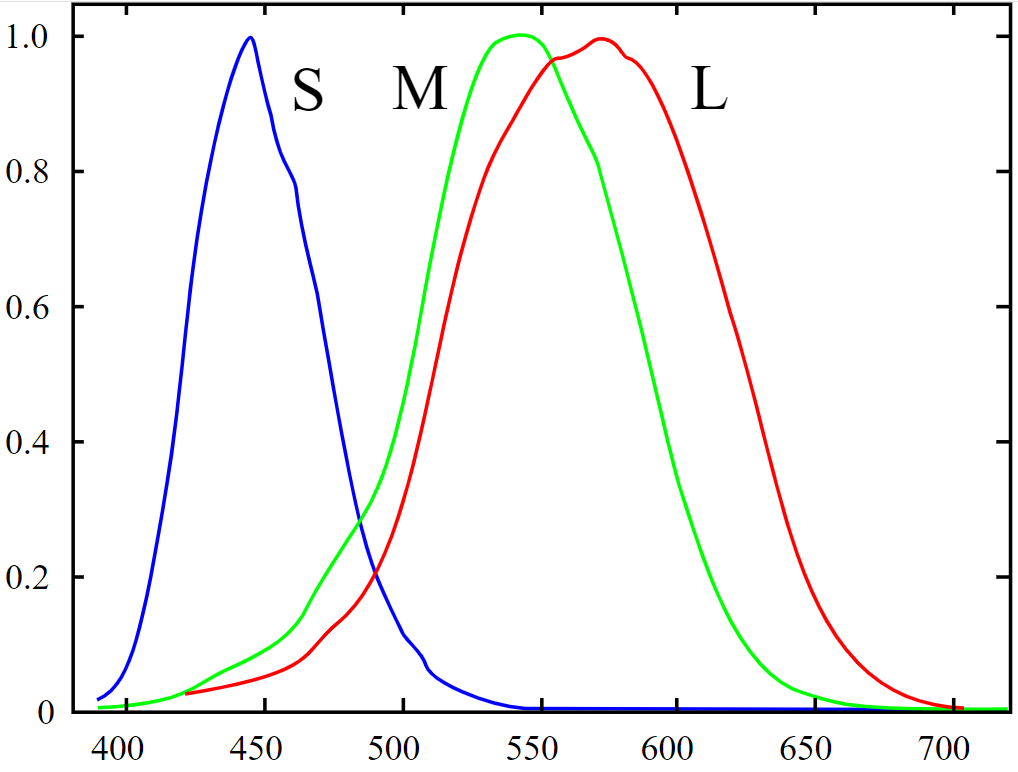
\includegraphics[angle=0, width=5.5cm]{Images/experimental/lms_coordinates.png}
                    %\label{Figure 1}
                \end{figure}
		\end{column}		
	\end{columns}
\end{frame}


 \begin{frame}{Experimentos de discriminación}{Calibración}
     Realizamos una calibración de la pantalla para realizar los experimentos de manera tal de obtener una transformación $\{\textbf{R,G,B}\} \Rightarrow \{\textbf{S,M,L}\}$, a través de
     \begin{equation*}
         C = \int_{-\infty}^{\infty}\, d\lambda \, E_{R,G,B}(\lambda) \, \alpha_C(\lambda) \,\text{       con }C  \in \{\textbf{S,M,L}\}
     \end{equation*}
     y un ajuste del tipo
     
     \begin{equation*}
    \begin{pmatrix}
        \mathbf{S} \\ 
        \mathbf{M} \\ 
        \mathbf{L}
    \end{pmatrix} = \begin{pmatrix}
        \alpha_{SR} & \alpha_{SG} & \alpha_{SB} \\ \alpha_{MR} & \alpha_{MG} & \alpha_{MB} \\ \alpha_{LR} & \alpha_{LG} & \alpha_{LB}  
    \end{pmatrix} \begin{pmatrix}
        \mathbf{R}^{\gamma_r} \\ 
        \mathbf{G}^{\gamma_g} \\ 
        \mathbf{B}^{\gamma_b}
    \end{pmatrix} + \begin{pmatrix}
        a_S \\ a_M \\ a_L
    \end{pmatrix},
\end{equation*}
\end{frame}

\begin{frame}{Experimentos de discriminación}{Resultados del ajuste}
    \begin{figure}
        \centering
        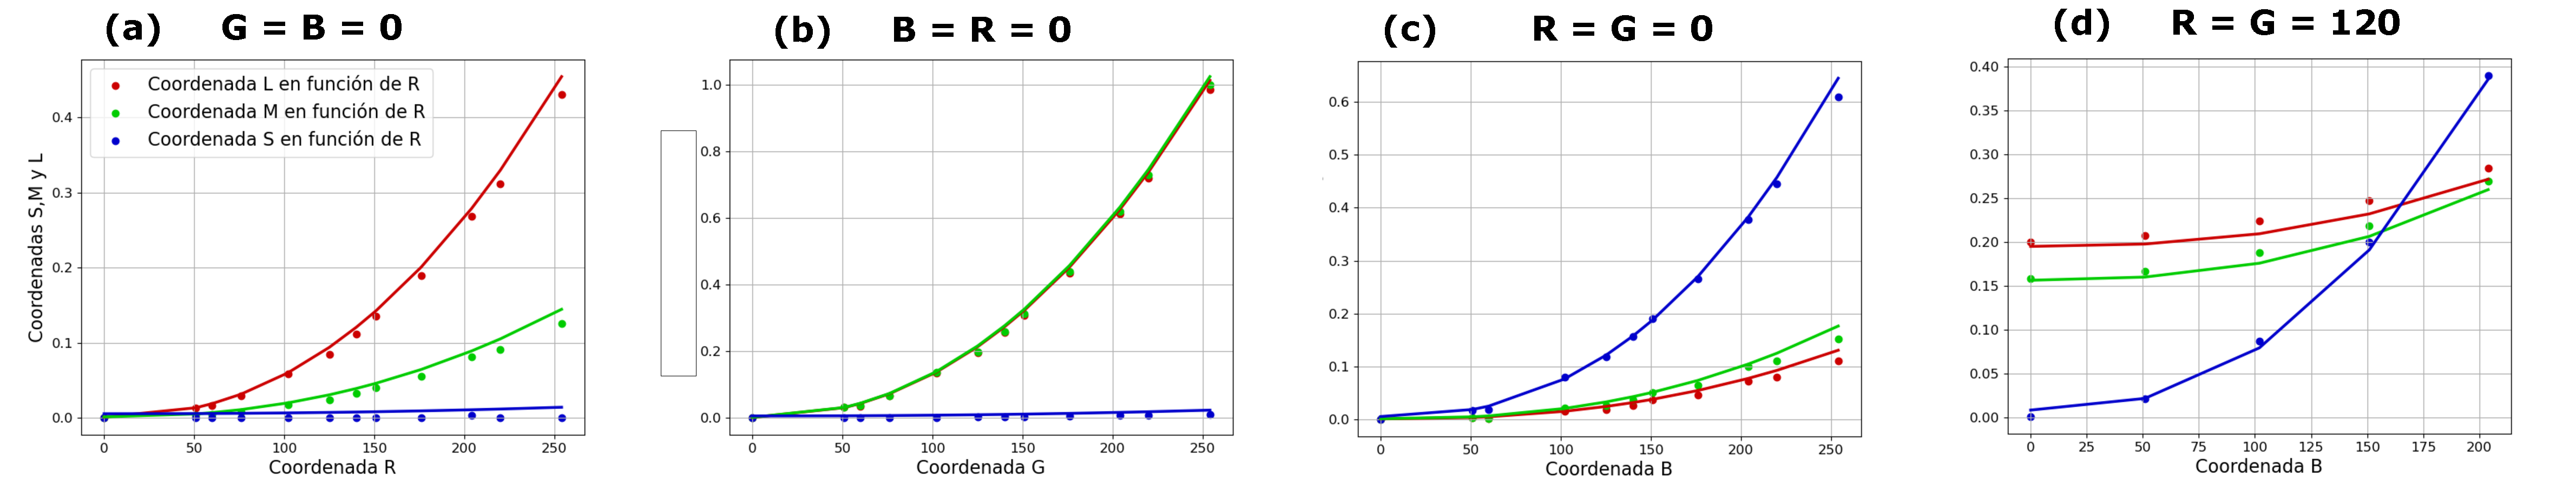
\includegraphics[width = 15cm]{Images/experimental/ajuste.pdf}
        %\caption{Caption}
        %\label{fig:enter-label}
    \end{figure}
\end{frame}


\begin{frame}{Experimentos de discriminación}{El estímulo}
Presentamos el siguiente estímulo a los voluntarios,
\begin{equation*}
     \mathbf{r}(x,y) = \mathbf{r_0} + \sqrt{k}\bm{\epsilon}\text{J}_0\left(k\sqrt{x^2+y^2}\right),
\end{equation*}
con su centro en cuatro posiciones posibles y $\bm{\epsilon}$ a lo largo de las direcciones $\mathbf{S}$, $\mathbf{L-M}$ y $\mathbf{L+M}$.
\begin{center}
    \begin{figure}[h]
     \centering
     \begin{subfigure}[b]{0.24\textwidth}
         \centering
         
\includegraphics[width=\textwidth]{Images/experimental/izquierda_charla.png}
         %\caption{Centro de la modulación a la izquierda del centro de la pantalla.}
         \label{fig:y equals x}
     \end{subfigure}
     \hfill
     \begin{subfigure}[b]{0.24\textwidth}
         \centering
         
\includegraphics[width=\textwidth]{Images/experimental/derecha_charla.png}
         %\caption{Centro de la modulación a la derecha del centro de la pantalla.}
         \label{fig:three sin x}
     \end{subfigure}
     \hfill
     \begin{subfigure}[b]{0.24\textwidth}
         \centering
         
\includegraphics[width=\textwidth]{Images/experimental/arriba_charla.png}
         %\caption{Centro de la modulación arriba del centro de la pantalla.}
         \label{fig:five ovr x}
     \end{subfigure}
     \hfill  
     \begin{subfigure}[b]{0.24\textwidth}
         \centering
         
\includegraphics[width=\textwidth]{Images/experimental/abajo_charla.png}
         %\caption{Centro de la modulación abajo del centro de la pantalla.}
         \label{fig:fve over x}
     \end{subfigure}
     %\caption{Diferentes centrados del estímulo presentado.}
     \label{fig:cap2_estimulo}
\end{figure} 
\end{center}
\end{frame}
%---------------------------------
\begin{frame}{Experimentos de discriminación}{La tarea}
    \begin{itemize}
        \item Se fija la frecuencia $k$ y la dirección de la modulación $\bm{\hat{\epsilon}}$.\pause
        \item Se le presenta al voluntario un punto negro en el centro de la pantalla durante 2 segundos.\pause
        \item Se le presenta el estímulo con una amplitud $\epsilon$ descentrado al voluntario durante 1 segundo.\pause
        \item Se le pide al voluntario que eliga con las flechas del teclado la posición del centro, o que responda al azar en caso de que no haya percibido el estímulo. \pause
        \item Se repite el procedimiento un total de 50 veces cambiando el valor de la amplitud.
    \end{itemize}        
\end{frame}


%-------------------------------------------------------
\begin{frame}{Experimentos de discriminación}{Probabilidad de acierto y error}
    \onslide<1->
    Propusimos que la probabilidad de que una persona se equivoque ($x=0$) o acierte ($x=1$) la posición del centro, dado $h(k)$ y $\epsilon$, es

\begin{columns}[c]

\begin{column}{0.5\textwidth}
    

    
    \begin{equation*}\label{eqn:cap2_prob}
P(x|\epsilon,h)=
    \begin{cases}
        \displaystyle\frac{3}{4}\exp\left[-(\epsilon/h(k))^2\right] & \text{si } x = 0\\
        1 - \displaystyle\frac{3}{4}\exp\left[-(\epsilon/h(k))^2\right] & \text{si } x = 1.
    \end{cases}
\end{equation*}

\end{column}

\begin{column}{0.5\textwidth}
    \begin{figure}
        \centering
        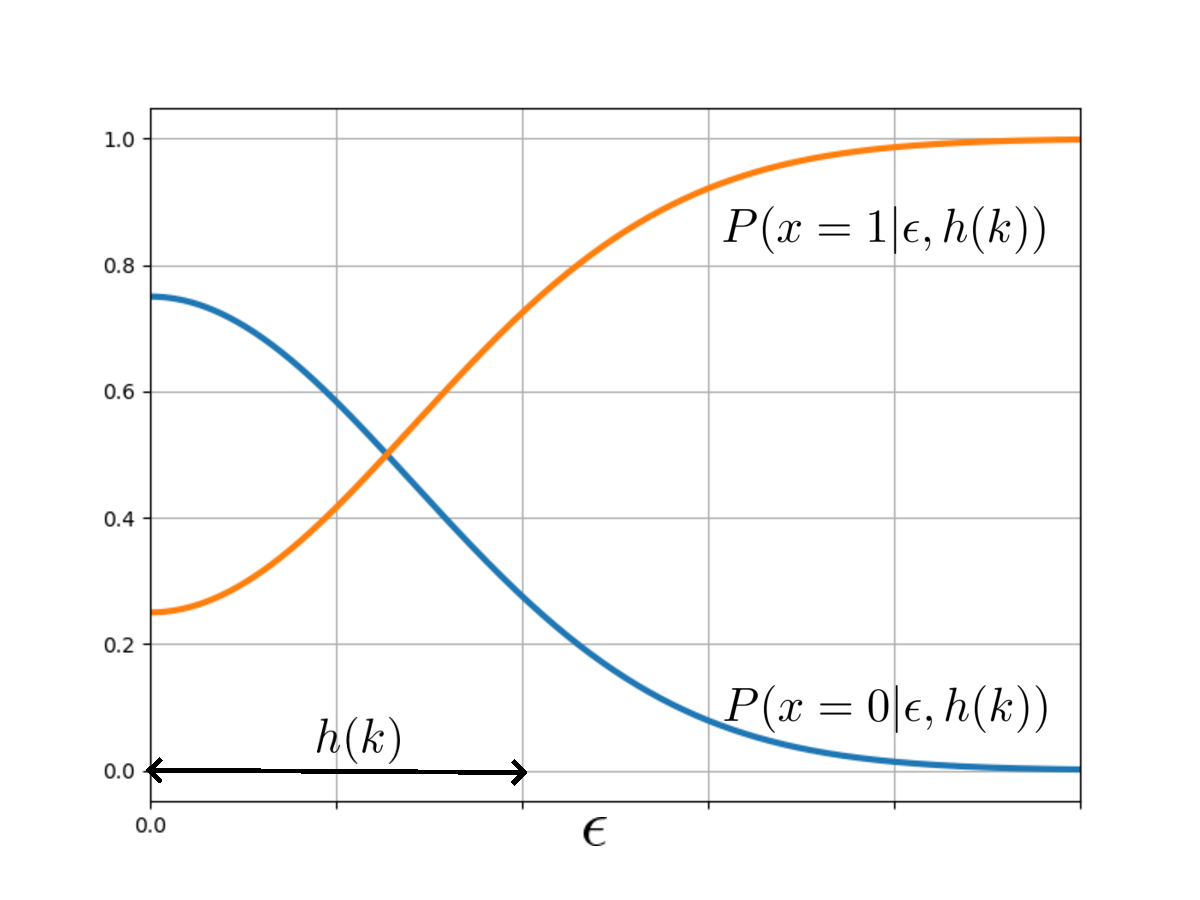
\includegraphics[width = 5cm]{Images/experimental/p_de_x_cuad.pdf}
        %\caption{Caption}
        %\label{fig:my_label}
    \end{figure}
    
\end{column}


\end{columns}

El umbral de discriminación $h(k)$ representa una amplitud característica del estímulo.


\end{frame}



%----------------------------------------------------------------
\begin{frame}{Experimentos de discriminación}{Estimación del umbral de discriminación}
Dado el conjunto $(x_1,x_2,\dots,x_n)$ de aciertos y errores, y un conjunto $(\epsilon_1,\epsilon_2,\dots,\epsilon_n)$ de amplitudes para un dado $k$ utilizamos el estimador de máxima verosimilitud para estimar el $h(k)$ del voluntario,
el cual consiste en maximizar el logaritmo de la función de verosimilitud
\vspace{1cm}
    \begin{align*}
    \text{log } \mathcal{L}(h) &= \text {log } \displaystyle\left[\prod_{j=1}^n P(x_j|\epsilon_j,h)\right] \\
     &= \displaystyle\sum_{j / x_j = 0} \text{log}\left(\displaystyle\frac{3}{4}\exp\left[-(\epsilon_j/h(k))^2\right]\right) + \displaystyle\sum_{j/x_j = 1}\text{log}\left(1 - \displaystyle\frac{3}{4}\exp\left[-(\epsilon_j/h(k))^2\right]\right)
    \end{align*}
\end{frame}
%-----------------------------------------------------------
\begin{frame}{Experimentos de discriminación}{Muestreo de amplitudes}
    \onslide<1->\begin{block}{}
   Mostrar amplitudes muestreadas de una distribución uniforme no es óptimo.
    	\end{block}
\onslide<2->\begin{block}{}
    ¿Cómo aprovechar la información que conseguimos en cada trial para acelerar la convergencia al valor del umbral?
    	\end{block}
\onslide<3->\begin{block}{Idea:}
    \centering 
    Maximizar la información de Fisher $J(h|\epsilon)$ de la distribución respecto a la amplitud $\epsilon$.
    	\end{block}

\end{frame}
%--------------------------------------------------
\begin{frame}{Experimentos de discriminación}{Maximización de la información de Fisher}
    La información de Fisher $J(h|\epsilon)$ está definida como 
    \begin{equation*}
        J(h|\epsilon) = -\displaystyle\left\langle\frac{\partial^2}{\partial h^2} \text{log }p(x|h,\epsilon) \right\rangle,
    \end{equation*}
 y representa qué tan informativa es una muestra $x$ para estimar el valor de $h$. \pause
\centering
\\
 Maximizando $J(h|\epsilon)$ respecto $\epsilon$ obtenemos \\
     $\epsilon_{n+1} = \alpha h_n \text{  con  } \alpha \approx 1.317$.


\end{frame}
%--------------------------------------------------

\begin{frame}{Experimentos de discriminación}{Comprobación de la maximización}

\begin{columns}[c] % The "c" option specifies centered vertical alignment while the "t" option is used for top vertical alignment

    
		\begin{column}{0.40\textwidth}

    \begin{itemize}
        \item Se simuló un sujeto virtual que contestaba $x = 0$ o $x = 1$ dado un valor de $h$ y amplitudes $\epsilon$.
        \item En un promedio de 20 realizaciones se observa que el método adaptativo converge más rápidamente.
        \item El error promedio en el paso 50 en 1600 realizaciones se minimiza en $\alpha \approx 1.317$.
    \end{itemize}

          
 
               
		\end{column}
  		\begin{column}{0.60\textwidth} % Left column width
                \onslide<1-> \begin{figure}[h!]
                    \centering
                    %\caption{Hawkins et al, 2015}
                    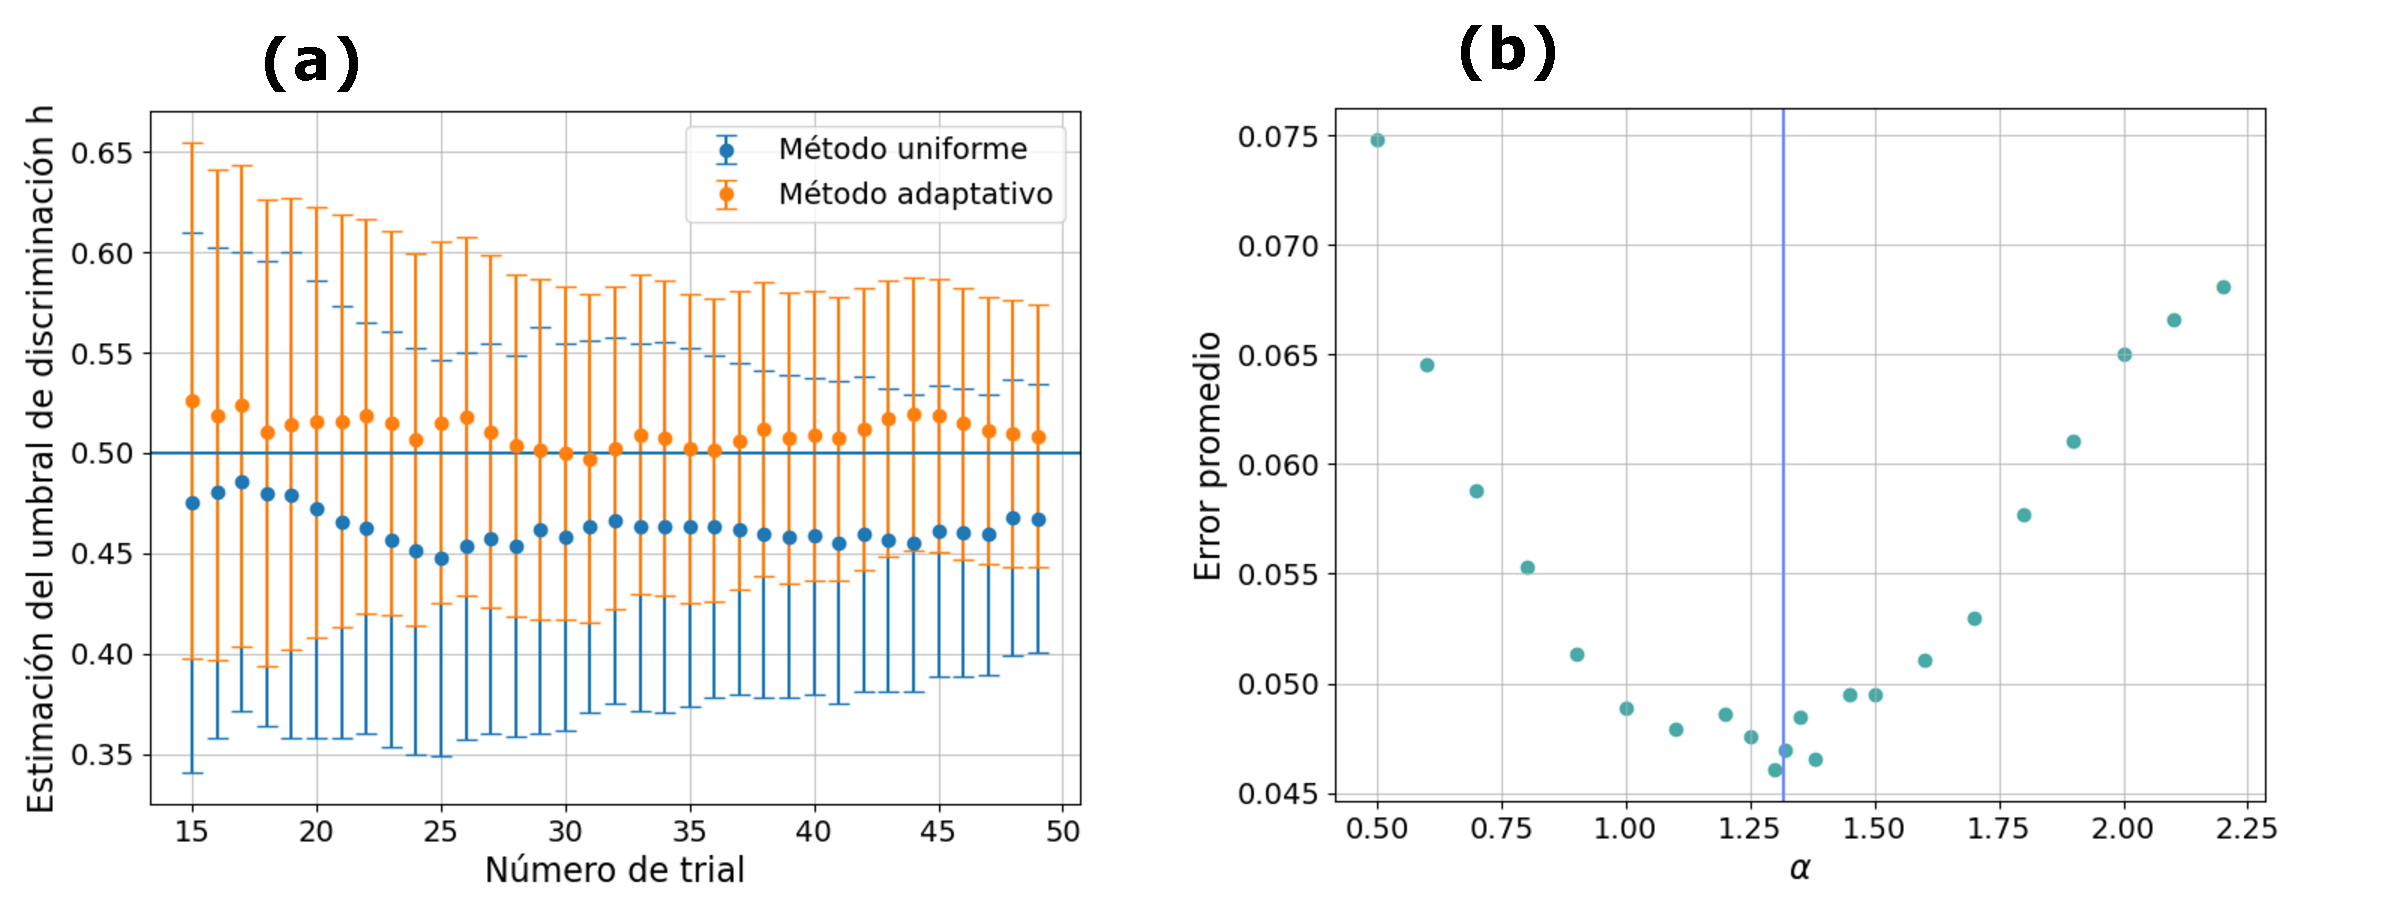
\includegraphics[angle=0, width=9.0cm]{Images/experimental/comparacion_y_alfas.pdf}
                    %\label{Figure 1}
                \end{figure}
		\end{column}		
	\end{columns}
    
\end{frame}
%---------------------------------------------------------------
\begin{frame}{Experimentos de discriminación}{Protocolo experimental}
    \begin{itemize}
        \item Se midieron los umbrales de discriminación en 7 voluntarios. \pause
        \item Cada voluntario hizo 100 iteraciones para 5 valores de frecuencia espacial $k$ en promedio. \pause
        \item 3 voluntarios midieron solo en la dirección \textbf{S}, 2 midieron en las direcciones \textbf{S} y \textbf{L + M},
            y 2 midieron en las direcciones \textbf{S}, \textbf{L + M} y \textbf{L - M}. 
    \end{itemize}
\end{frame}
%----------------------------------------------------------------






\begin{frame}
    \begin{center}
        \Huge \textbf{\textcolor{orange}{Resultados}}

    \end{center}
    % Aquí puedes agregar el resto del contenido de tu frame
\end{frame}






%---------------------------------------------------------------
\begin{frame}{Resultados}{Algunas curvas de umbrales de discriminación: Eje S}
    \begin{columns}[c] % The "c" option specifies centered vertical alignment while the "t" option is used for top vertical alignment

    
		\begin{column}{0.50\textwidth} % Right column width
            \begin{center}
                Voluntarie B: \\ $k_{\text{min}} = (0.41 \pm 0.01)\frac{1}{\text{grados}}$ \\ $\sigma = (2.43 \pm 0.06)^\circ$
            \end{center}
            
               
                    \onslide<1-> \begin{figure}[h!]
                    \centering
                    %\caption{Hawkins et al, 2015}
                    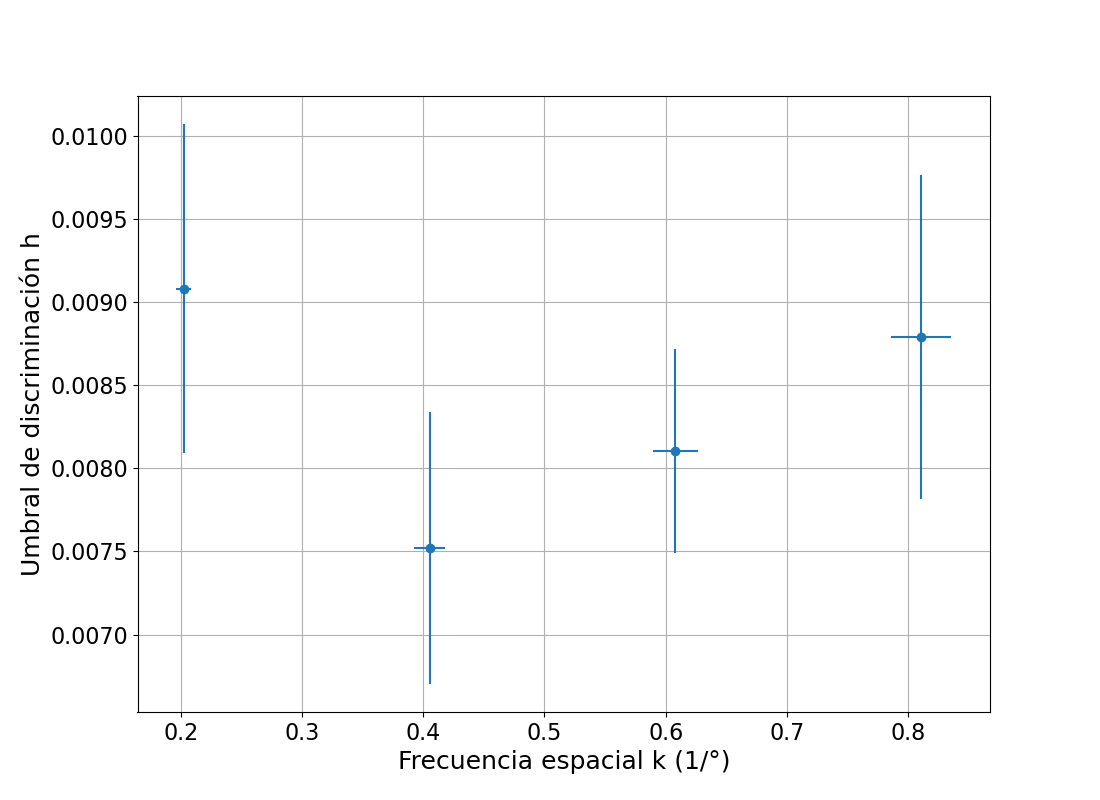
\includegraphics[angle=0, width=5cm]{Images/resultados/bauti_s.png}
                    %\label{Figure 1}
                \end{figure}
               
        
               
		\end{column}

    
  		\begin{column}{0.50\textwidth} % Left column width
            \begin{center}
                Voluntarie M: \\ $k_{\text{min}} = (0.48 \pm 0.02)\frac{1}{\text{grados}}$ \\ $\sigma = (2.05 \pm 0.08)^\circ$
            \end{center}
                \onslide<1-> \begin{figure}[h!]
                    \centering
                    %\caption{Hawkins et al, 2015}
                    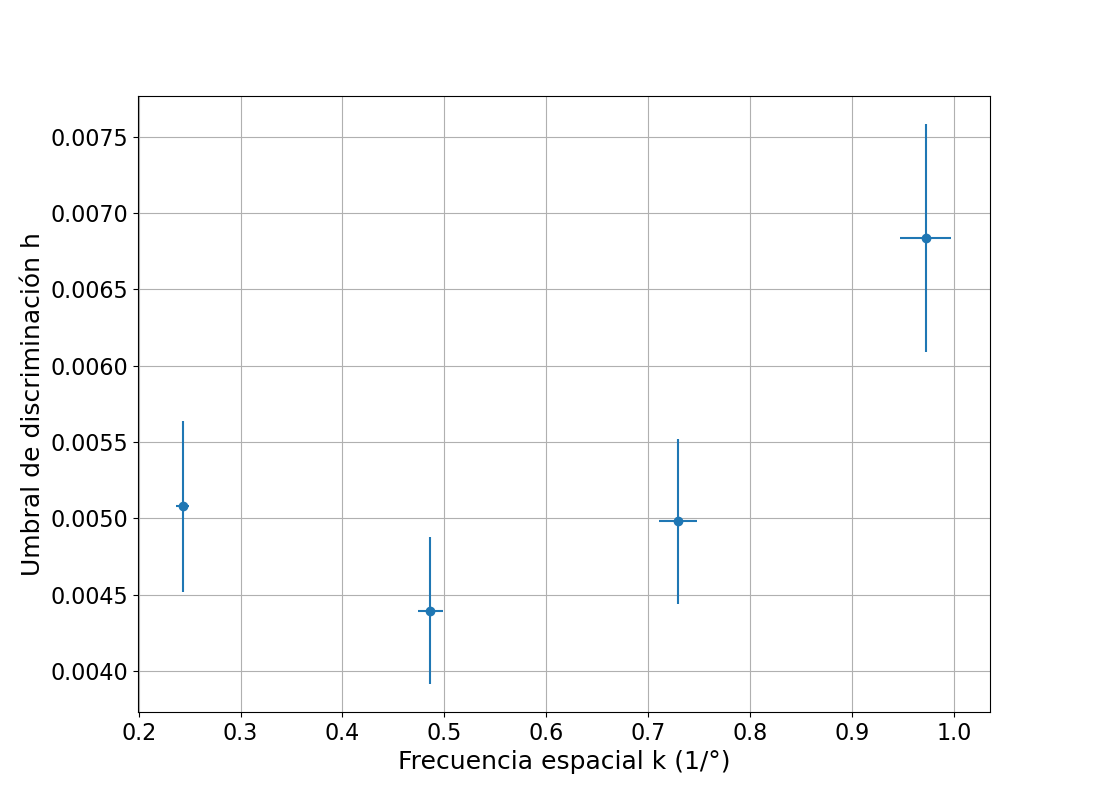
\includegraphics[angle=0, width=5cm]{Images/resultados/martina_s.png}
                    %\label{Figure 1}
                \end{figure}
		\end{column}		
	\end{columns}

\end{frame}
%----------------------------------------------------
\begin{frame}{Resultados}{Eje S y L+M}
    \begin{columns}[c] % The "c" option specifies centered vertical alignment while the "t" option is used for top vertical alignment

    
		\begin{column}{0.50\textwidth} % Right column width
            \begin{center}
                Voluntarie I: \\ $k_{\text{min}} = (0.43 \pm 0.03)\frac{1}{\text{grados}}$ \\ $\sigma = (2.3 \pm 0.2)^\circ$
            \end{center}  
                    \onslide<1-> \begin{figure}[h!]
                    \centering
                    %\caption{Hawkins et al, 2015}
                    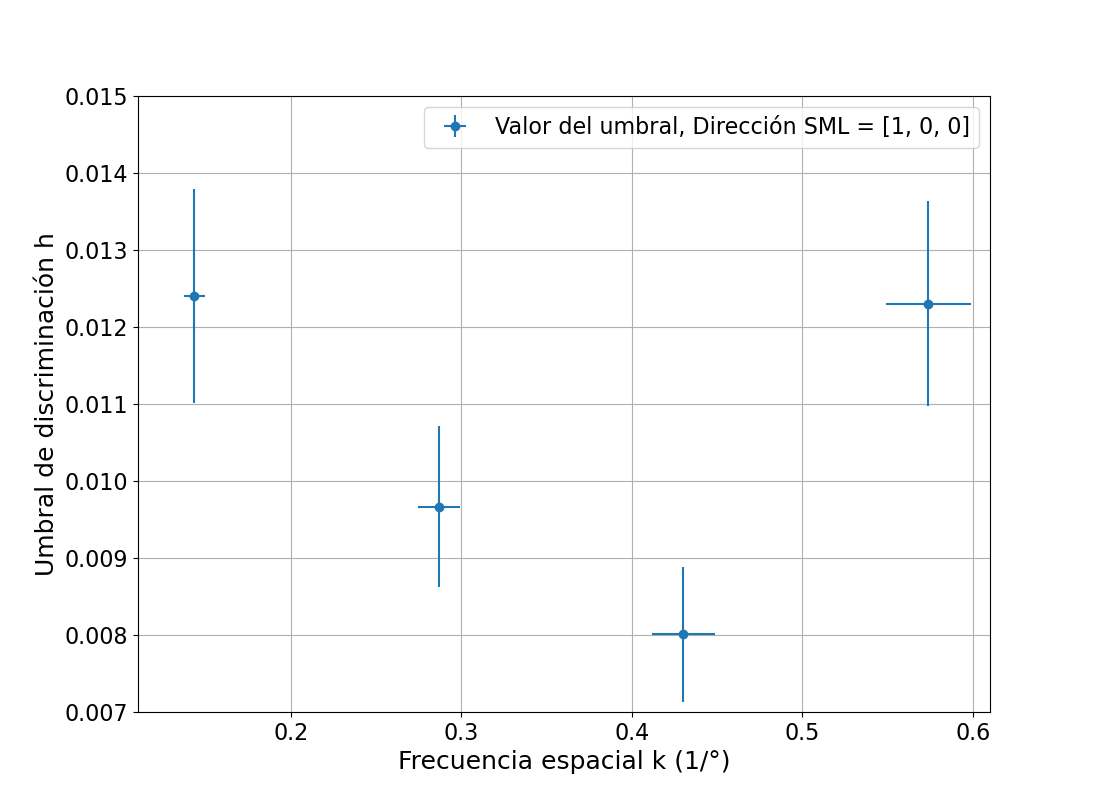
\includegraphics[angle=0, width=5cm]{Images/resultados/ines_s.png}
                    %\label{Figure 1}
                \end{figure}
               
        
               
		\end{column}

    
  		\begin{column}{0.50\textwidth} % Left column width
            \begin{center}
                Voluntarie I: \\ $k_{\text{min}} = (1.00 \pm 0.04)\frac{1}{\text{grados}}$ \\ $\sigma = (1.00 \pm 0.04)^\circ$
            \end{center}
                \onslide<1-> \begin{figure}[h!]
                    \centering
                    %\caption{Hawkins et al, 2015}
                    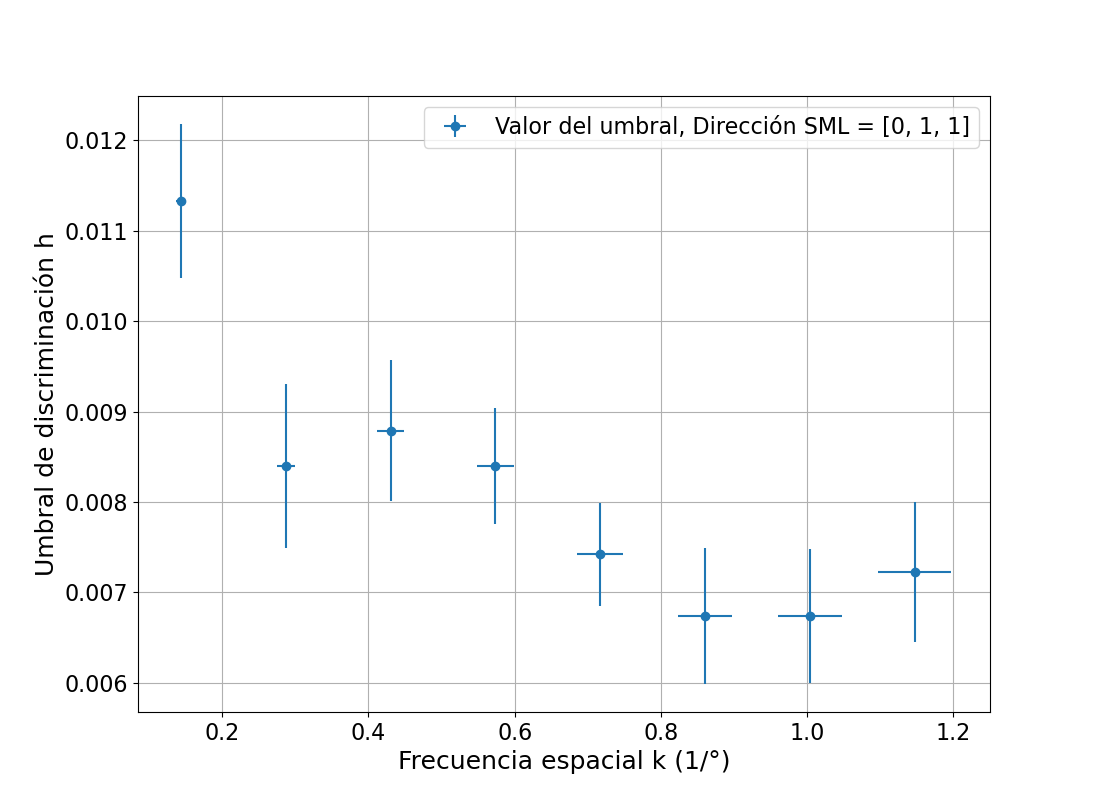
\includegraphics[angle=0, width=5cm]{Images/resultados/ines_l_mas_m.png}
                    %\label{Figure 1}
                \end{figure}
		\end{column}		
	\end{columns}

\end{frame}

\begin{frame}{Resultados}{Eje S con diferentes fondos}
    \begin{columns}[c] % The "c" option specifies centered vertical alignment while the "t" option is used for top vertical alignment

    
		\begin{column}{0.50\textwidth} % Right column width
        \begin{center}
            Voluntarie T: $SML_\text{fondo} = [0.13, 0.30, 0.35]$\\ $k_{\text{min}} = (0.59 \pm 0.03)\frac{1}{\text{grados}}$ \\ $\sigma = (1.69 \pm 0.08)^\circ$
        \end{center}    
                    \onslide<1-> \begin{figure}[h!]
                    \centering
                    %\caption{Hawkins et al, 2015}
                    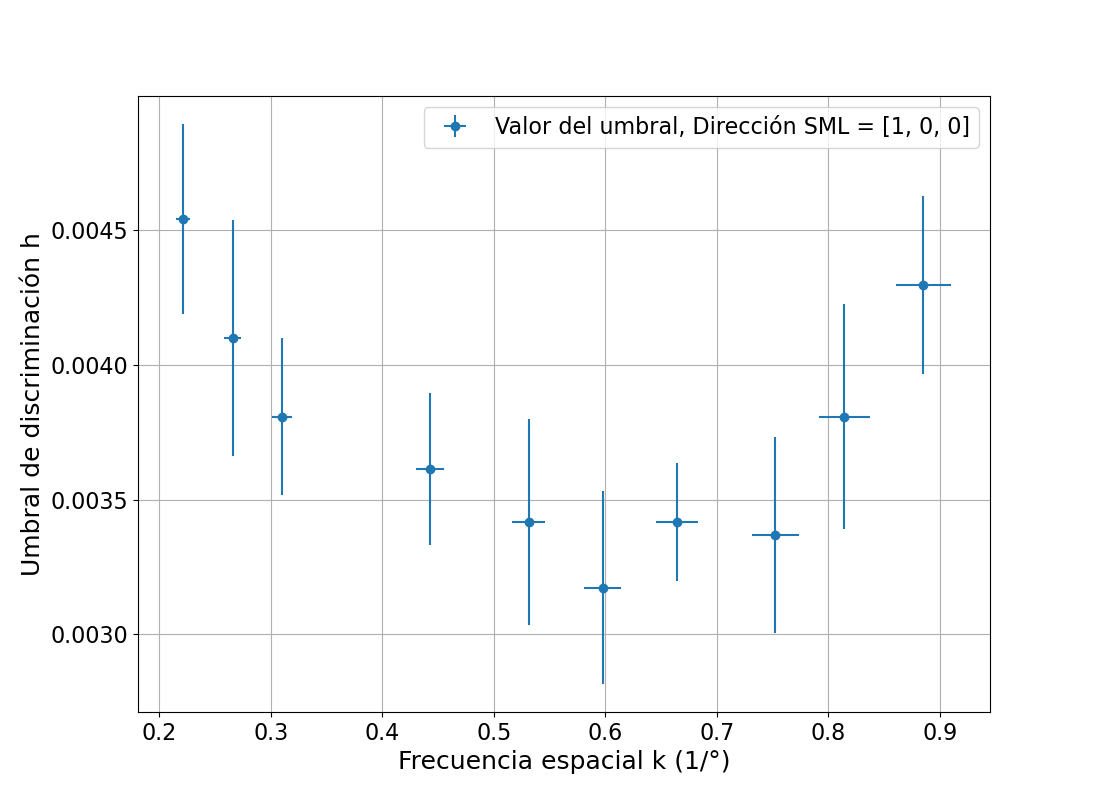
\includegraphics[angle=0, width=5cm]{Images/resultados/s_yo_gris.png}
                    %\label{Figure 1}
                \end{figure}
               
        
               
		\end{column}

    
  		\begin{column}{0.50\textwidth} % Left column width
            \begin{center}
                $SML_\text{fondo} = [0.25, 0.30, 0.35]$\\ $k_{\text{min}} = (0.59 \pm 0.08)\frac{1}{\text{grados}}$ \\ $\sigma = (1.7 \pm 0.2)^\circ$
            \end{center}
                \onslide<1-> \begin{figure}[h!]
                    \centering
                    %\caption{Hawkins et al, 2015}
                    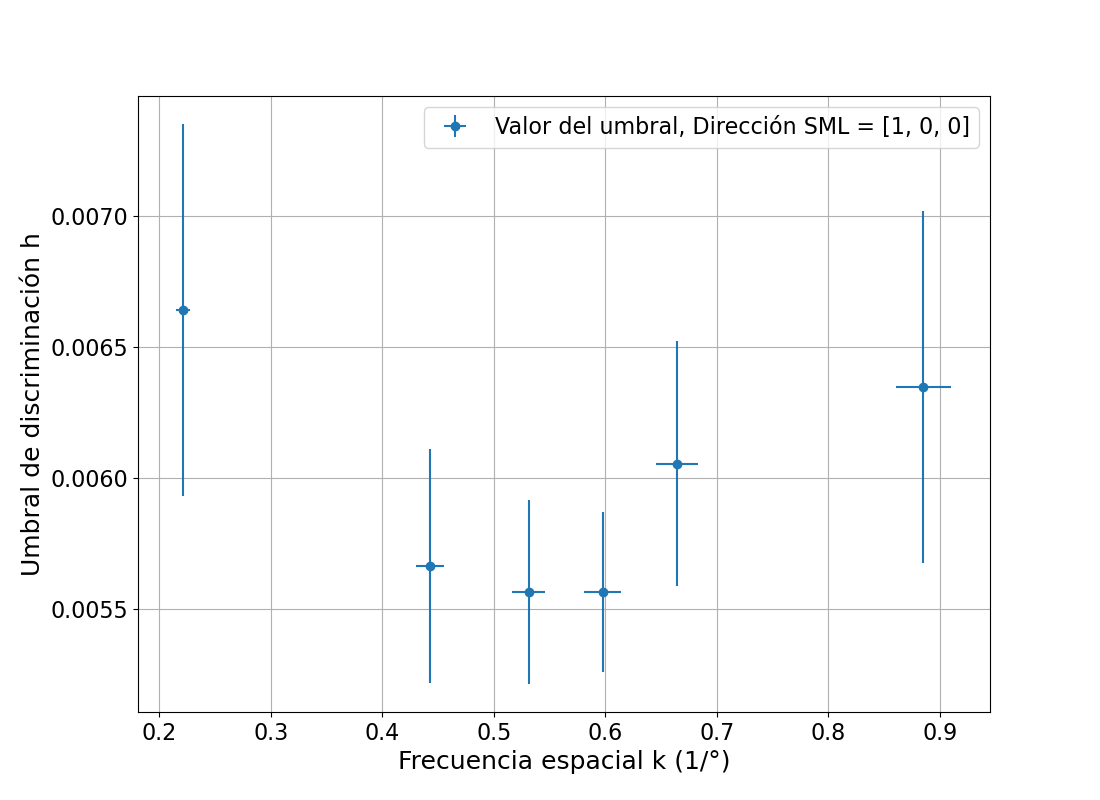
\includegraphics[angle=0, width=5cm]{Images/resultados/s_yo_gris_azulado.png}
                    %\label{Figure 1}
                \end{figure}
		\end{column}		
	\end{columns}

\end{frame}

\begin{frame}{Resultados}{Eje L + M y L - M}
    \begin{columns}[c] % The "c" option specifies centered vertical alignment while the "t" option is used for top vertical alignment

    
		\begin{column}{0.50\textwidth} % Right column width
            \begin{center}
                Voluntarie T: \\ $k_{\text{min}} = (1.75 \pm 0.04)\frac{1}{\text{grados}}$ \\ $\sigma = (0.57 \pm 0.02)^\circ$
            \end{center}
                    \onslide<1-> \begin{figure}[h!]
                    \centering
                    %\caption{Hawkins et al, 2015}
                    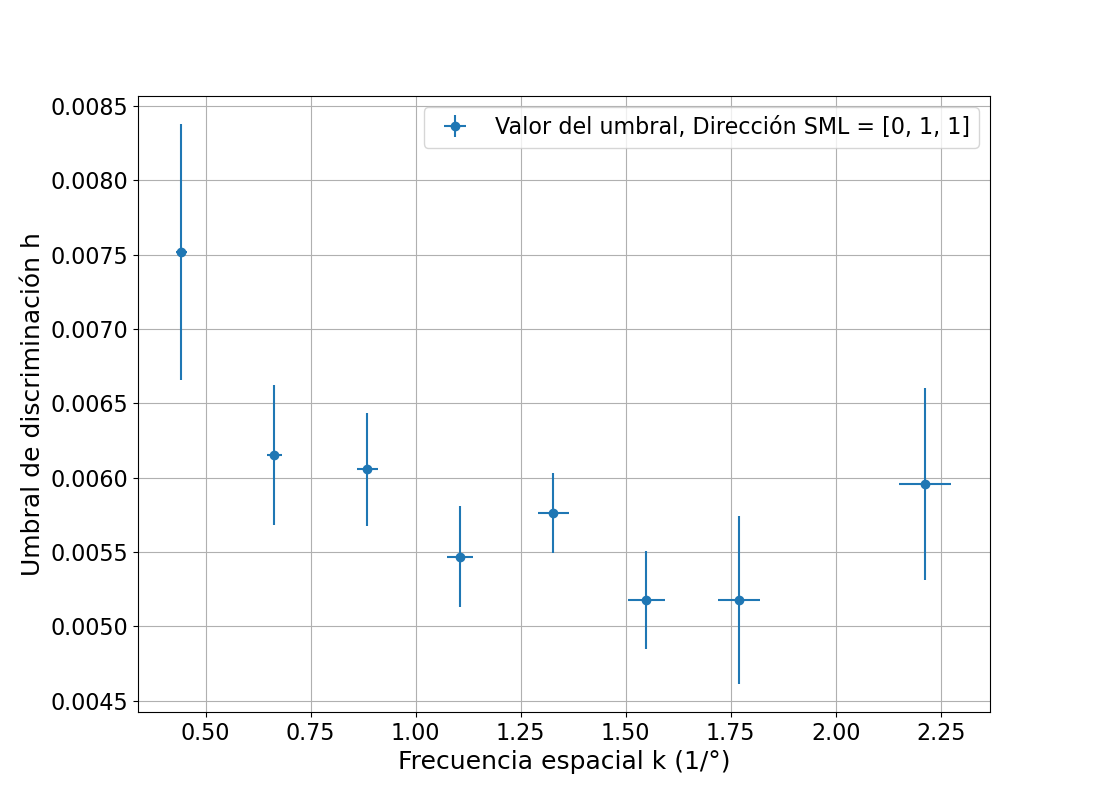
\includegraphics[angle=0, width=5cm]{Images/resultados/l_mas_m_yo.png}
                    %\label{Figure 1}
                \end{figure}
               
        
               
		\end{column}

    
  		\begin{column}{0.50\textwidth} % Left column width
            \begin{center}
                $k_\text{min} = (0.62 \pm 0.06)\frac{1}{\text{grados}}$ \\ $\sigma = (1.6 \pm 0.2)^\circ$
            \end{center}
                \onslide<1-> \begin{figure}[h!]
                    \centering
                    %\caption{Hawkins et al, 2015}
                    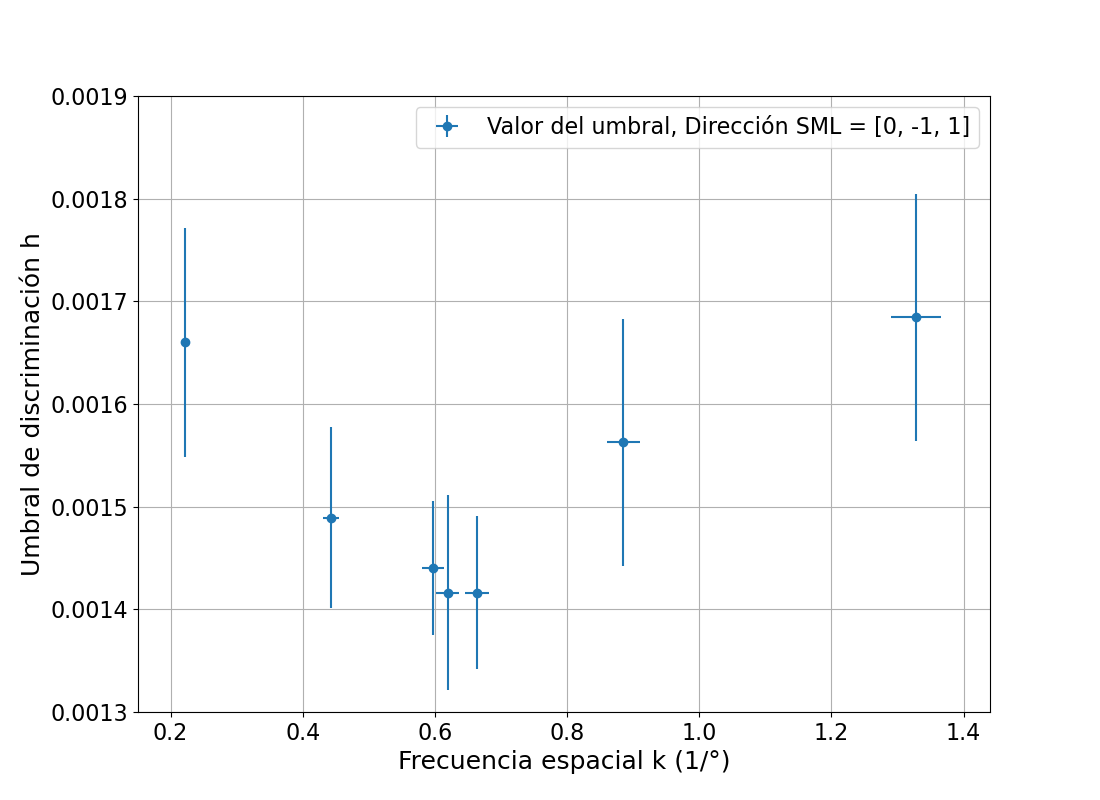
\includegraphics[angle=0, width=5cm]{Images/resultados/l_menos_m_yo.png}
                    %\label{Figure 1}
                \end{figure}
		\end{column}		
	\end{columns}

\end{frame}


\begin{frame}{Resultados}
    \begin{columns}[c] % The "c" option specifies centered vertical alignment while the "t" option is used for top vertical alignment

    
		\begin{column}{0.50\textwidth}

    \begin{itemize}
        \item Se realizaron experimentos en 7 voluntarios, donde, para cada uno de ellos y cada dirección medida se encontraron mínimos de discriminación.
        \item Las frecuencias óptimas en los ejes $\mathbf{S}$ y \textbf{L - M} son similares, mientras que en el eje \textbf{L + M} toman valores mayores.
      
    \end{itemize}

                
		\end{column}
  		\begin{column}{0.50\textwidth} % Left column width
                \onslide<1-> \begin{figure}[h!]
                    \centering
                    %\caption{Hawkins et al, 2015}
                    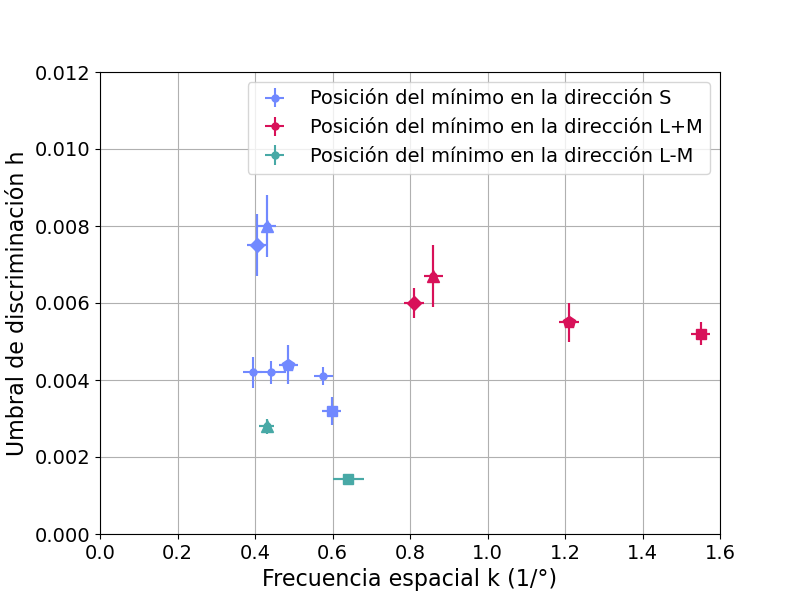
\includegraphics[angle=0, width=6.5cm]{Images/resultados/minimos_fondo_128_128_128.png}
                    %\label{Figure 1}
                \end{figure}
		\end{column}		
	\end{columns}
\end{frame}




\begin{frame}{Resultados}
    \begin{columns}[c] % The "c" option specifies centered vertical alignment while the "t" option is used for top vertical alignment

    
		\begin{column}{0.40\textwidth}

   \begin{itemize}
        \item Para los voluntarios que midieron en $\mathbf{S}$ y \textbf{L - M} se obtuvieron los mismos valores de frecuencia óptima.
        \item Las frecuencias óptimas en \textbf{L + M} son aproximadamente el doble que en la dirección \textbf{S}.
      
    \end{itemize}

                
		\end{column}
  		\begin{column}{0.60\textwidth} % Left column width
                \onslide<1-> \begin{figure}[h!]
                    \centering
                    %\caption{Hawkins et al, 2015}
                    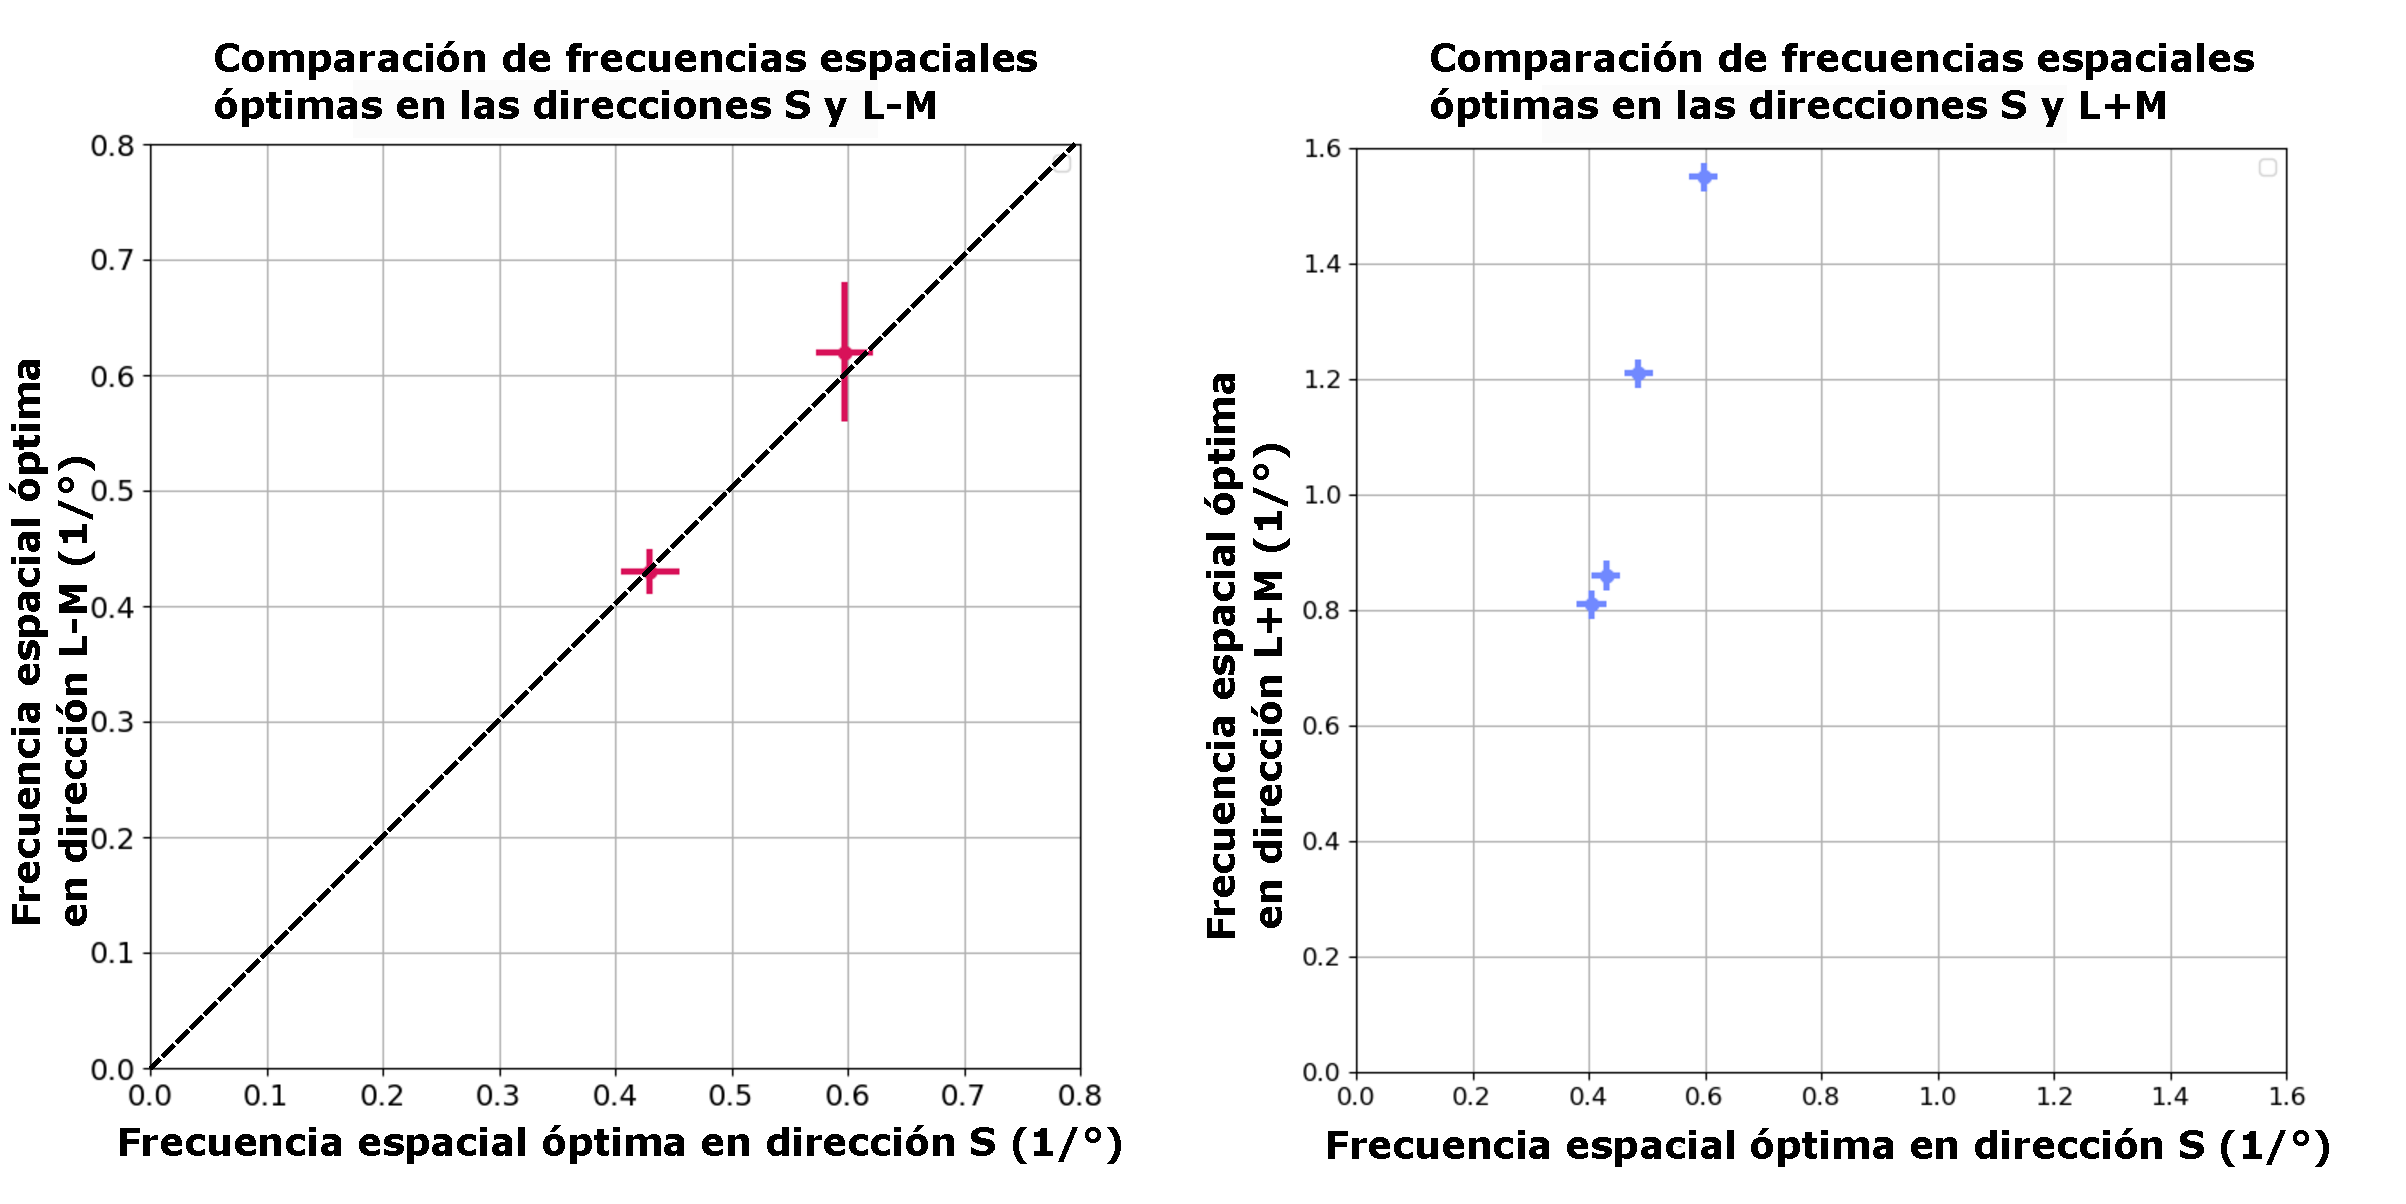
\includegraphics[angle=0, width=8.5cm]{Images/resultados/comparaciones_ar1_def.pdf}
                    %\label{Figure 1}
               \end{figure}
		\end{column}		
	\end{columns}
\end{frame}

\begin{frame}{Resultados}
  \begin{columns}[c] % The "c" option specifies centered vertical alignment while the "t" option is used for top vertical alignment

    
		\begin{column}{0.40\textwidth}

    \begin{itemize}
        \item El umbral de discriminación depende del valor del fondo. Según la ley de Weber, el umbral crece linealmente con este. 
        \item El valor del umbral en la dirección \textbf{S} aumenta linealmente con el valor \textbf{S} del fondo utilizado.
      
    \end{itemize}

                
		\end{column}
  		\begin{column}{0.60\textwidth} % Left column width
                \onslide<1-> \begin{figure}[h!]
                    \centering
                    %\caption{Hawkins et al, 2015}
                    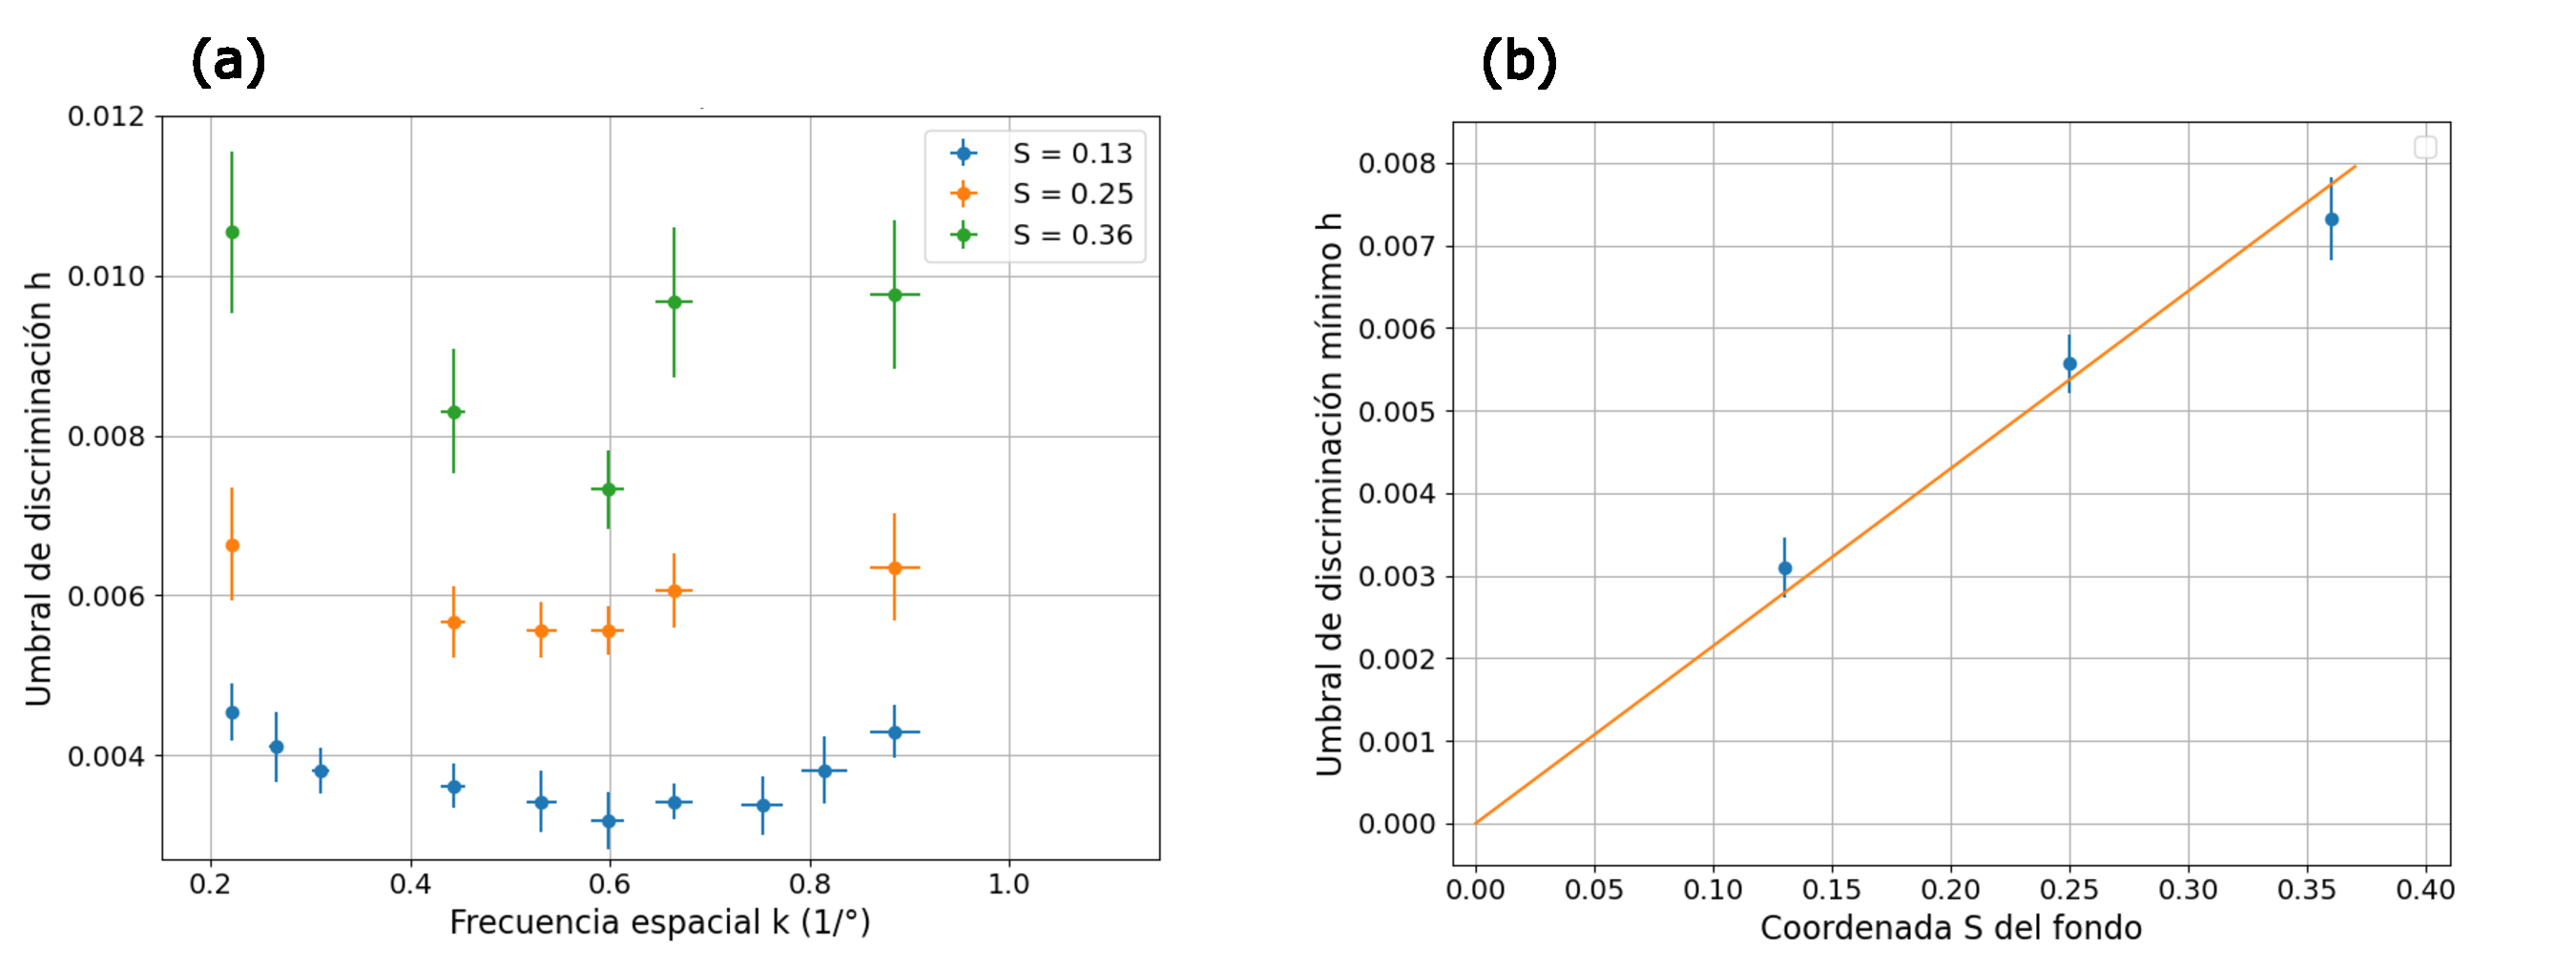
\includegraphics[angle=0, width=8.5cm]{Images/resultados/ley_weber_s.pdf}
                    %\label{Figure 1}
                \end{figure}
		\end{column}		
	\end{columns}
    
\end{frame}

\begin{frame}{Resultados}
    \begin{columns}[c] % The "c" option specifies centered vertical alignment while the "t" option is used for top vertical alignment

    
		\begin{column}{0.50\textwidth}

    \begin{itemize}
        \item Para comparar umbrales en diferentes direcciones utilizamos el \textit{umbral normalizado}, la pendiente dada por la ley de Weber $\frac{h_\mathbf{\alpha}}{c_\mathbf{\alpha}}$. 
        \item En ambos sujetos que midieron en las tres direcciones se observa que el umbral normalizado toma su menor valor en la dirección \textbf{L + M}.
      
    \end{itemize}

                
		\end{column}
  		\begin{column}{0.50\textwidth} % Left column width
                \begin{table}[h]
    \centering
    \begin{tabular}{cccc}
        \hline
        Sujeto &  $\frac{h_\mathbf{S}}{c_\mathbf{S}}$& $\frac{h_\mathbf{L - M}}{c_\mathbf{L - M}}$ & $\frac{h_\mathbf{L + M}}{c_\mathbf{L + M}}$\\
        \hline
        T & 0.024 & 0.034  & 0.011 \\ 
        I & 0.062 & 0.067 & 0.015\\
    \end{tabular}
%\caption{.}
\end{table}

\makebox[2.0cm]{}Coordenadas del fondo \\ 
\makebox[2.0cm]{}$\mathbf{LMS} = \{0.13,0.30,0.35\}$.
		\end{column}		
	\end{columns}
\end{frame}




\begin{frame}{Resultados}{En resumen}
    \begin{itemize}
        \onslide<1->\item Se hallaron mínimos para el umbral de discriminación $h$.
        \onslide<2->\item La frecuencia característica en la dirección de la componente lumínica del estímulo (\textbf{L+M}) es mayor que la frecuencia característica en las componentes cromáticas (\textbf{S} y \textbf{L - M}).
        \onslide<3->\item En los ejes cromáticos parece haber la misma frecuencia espacial característica.
        \onslide<4->\item El umbral cambia dependiendo del fondo linealmente en cierto rango (ley de Weber).
        \onslide<5->\item El umbral normalizado es menor en la dirección de la componente lumínica del estímulo que en sus componentes cromáticas.
        
    \end{itemize}
\end{frame}








%------------------------------------------------------
\section{Conclusiones}
%------------------------------------------------------
\begin{frame}{Conclusiones}
    \onslide<1->\begin{block}{}
    Modelamos a la red neuronal a cargo de procesar la inducción cromática como un campo receptivo con parámetros característicos.
    	\end{block}
\onslide<2->\begin{exampleblock}{}
    Dedujimos que, para acceder a estos parámetros del campo receptivo, debemos presentar un estímulo cuya cromaticidad debe ser modelado por una función de Bessel $\text{J}_0$.		
      
      
    	\end{exampleblock}

\onslide<3->\begin{alertblock}{}
            Diseñamos y llevamos a cabo experimentos perceptuales en siete voluntarios y obtuvimos distancias características para aproximadamente $2^\circ$ (eje S y L-M) y $0.75^\circ$ (eje L+M).
    	\end{alertblock}

\end{frame}

\begin{frame}{Conclusiones}
\onslide<1->\begin{block}{}
    Observamos que el umbral de discriminación es menor en la dirección de la componente lumínica del estímulo (\textbf{L + M}) que en sus componentes cromáticas (\textbf{S} y \textbf{L - M}).
    	\end{block}

\onslide<2->\begin{exampleblock}{}
    La frecuencia característica del eje \textbf{L + M} es mayor a la del eje \textbf{S} y \textbf{L - M}.
    	\end{exampleblock}

\onslide<3->\begin{alertblock}{}
    El umbral de discriminación depende del valor del fondo linealmente en cierto rango (ley de Weber).
    	\end{alertblock}
        
\end{frame}

%\begin{frame}{Trabajo a futuro}{Posible generalización al caso 3D}
%   Ahora $\epsilon$ es un vector $\vec{\epsilon}$ de tres componentes y $h$ se convierte en un tensor $\bm{H}(\vec{c})$, donde el valor del umbral depende del color $\vec{c}$ a partir de cual estamos sumando la modulación y de la dirección de la modulación.
%\vspace{1cm}

   
%   \centering
%   $ P(x|\vec{c},\vec{\epsilon},\bm{H})=
%    \begin{cases}
%        \displaystyle\frac{3}{4}\exp\left({-\frac{1}{2}\vec{\epsilon}^\text{t}\left[\bm{H}(\vec{c})^{-1}\right] \vec{\epsilon}}\right) & \text{si } x = 0\\
%        1 - \displaystyle\frac{3}{4}\exp\left({-\frac{1}{2}\vec{\epsilon}^\text{t}\left[\bm{H}(\vec{c})^{-1}\right] \vec{\epsilon}}\right) & \text{si } x = 1
%    \end{cases} $
%\end{frame}

%\begin{frame}{Trabajo a futuro}{Posible generalización al caso 3D}
%Los elipsoides representan superficies de probabilidad constante en el espacio de colores.
%    \begin{figure}
%        \centering
%        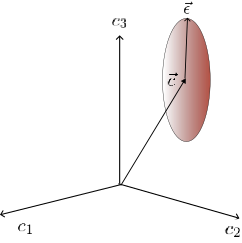
\includegraphics[width = 4cm]{Images/elipsoide.png}
        %\caption{Caption}
        %\label{fig:my_label}
%    \end{figure}
%\end{frame}

    	

%---------------------------------------------------------
%	CLOSING SLIDE
%---------------------------------------------------------

% To remove miniframe from top
%\appendix
\setbeamertemplate{headline}{}
\addtobeamertemplate{frametitle}{\vspace*{-\headheight}}{}

\begin{frame}[noframenumbering] %So the end and appendix slides don't contribute to the page count
%[plain] % The optional argument 'plain' hides the headline and footline
	%\frametitle{Questions?}

	\begin{center}
            {\LARGE ¿Preguntas?}
	\end{center}
 
\end{frame}
%---------------------------------------------------------

%------------------------------------------------

%------------------------------------------------


%------------------------------------------------


%------------------------------------------------

\end{document} 